%% LLT: Turn off some annoying warnings...

\RequirePackage{silence}
\WarningFilter{titlesec}{Non standard sectioning command}
\WarningFilter{scrreprt}{Usage of package}
\WarningFilter{scrreprt}{Activating an ugly workaround}

% **************************************************
% Document Class Definition
% **************************************************
\documentclass[%
	paper=A4,					% paper size --> A4 is default in Germany
	twoside=true,				% onesite or twoside printing
	openall,					% doublepage cleaning ends up right side
	parskip=full,				% spacing value / method for paragraphs
	chapterprefix=true,			% prefix for chapter marks
	11pt,						% font size
	headings=normal,			% size of headings
	bibliography=totoc,			% include bib in toc
	listof=totoc,				% include listof entries in toc
	titlepage=on,				% own page for each title page
	captions=tableabove,		% display table captions above the float env
	draft=false,				% value for draft version
]{scrreprt}%

% **************************************************
% Debug LaTeX Information
% **************************************************
%\listfiles

% **************************************************
% Information and Commands for Reuse
% **************************************************
\title{CGM Study}

\newcommand{\thesisTitle}{The Clean Thesis Style}
\newcommand{\thesisName}{Hrishi Olickel and Hebe Hilhorst}
\newcommand{\thesisSubject}{Random Subject}
% \newcommand{\thesisDate}{August 26, 2015}
% \newcommand{\thesisVersion}{My First Draft}

\newcommand{\thesisFirstReviewer}{Jane Doe}
\newcommand{\thesisFirstReviewerUniversity}{\protect{Clean Thesis Style University}}
\newcommand{\thesisFirstReviewerDepartment}{Department of Clean Thesis Style}

\newcommand{\thesisSecondReviewer}{John Doe}
\newcommand{\thesisSecondReviewerUniversity}{\protect{Clean Thesis Style University}}
\newcommand{\thesisSecondReviewerDepartment}{Department of Clean Thesis Style}

\newcommand{\thesisFirstSupervisor}{Jane Doe}
\newcommand{\thesisSecondSupervisor}{John Smith}

\newcommand{\thesisUniversity}{\protect{Clean Thesis Style University}}
\newcommand{\thesisUniversityDepartment}{Department of Clean Thesis Style}
\newcommand{\thesisUniversityInstitute}{Institut for Clean Thesis Dev}
\newcommand{\thesisUniversityGroup}{Clean Thesis Group (CTG)}
\newcommand{\thesisUniversityCity}{City}
\newcommand{\thesisUniversityStreetAddress}{Street address}
\newcommand{\thesisUniversityPostalCode}{Postal Code}

% **************************************************
% Load and Configure Packages
% **************************************************
\usepackage[utf8]{inputenc}		% defines file's character encoding
\usepackage[english]{babel} % babel system, adjust the language of the content

\usepackage{float}

\usepackage[					% clean thesis style
	figuresep=colon,%
	sansserif=false,%
	hangfigurecaption=false,%
	hangsection=true,%
	hangsubsection=true,%
	colorize=full,%
	colortheme=bluemagenta,%
% LLT: Use biber if using UTF8 encoding
	bibsys=bibtex,%
% 	bibsys=biber,%
	bibfile=Zotero,%
	bibstyle=alphabetic,%
]{cleanthesis}

% \DeclareSourcemap{
%   \maps[datatype=bibtex]{
%     \map[overwrite=true]{
%       \step[fieldset=urldate, null]
%     }
%   }
% }

\hypersetup{					% setup the hyperref-package options
	pdftitle={\thesisTitle},	% 	- title (PDF meta)
	pdfsubject={\thesisSubject},% 	- subject (PDF meta)
	pdfauthor={\thesisName},	% 	- author (PDF meta)
	plainpages=false,			% 	-
	colorlinks=false,			% 	- colorize links?
	pdfborder={0 0 0},			% 	-
	breaklinks=true,			% 	- allow line break inside links
	bookmarksnumbered=true,		%
	bookmarksopen=true			%
}

% **************************************************
% Document CONTENT
% **************************************************
\begin{document}

% --------------------------
% rename document parts
% --------------------------
%\renewcaptionname{ngerman}{\figurename}{Abb.}
%\renewcaptionname{ngerman}{\tablename}{Tab.}
\renewcaptionname{english}{\figurename}{Fig.}
\renewcaptionname{english}{\tablename}{Tab.}

% --------------------------
% Front matter
% --------------------------
\pagenumbering{roman}			% roman page numbing (invisible for empty page style)
% \pagestyle{empty}				% no header or footers
% % !TEX root = ../thesis-example.tex
%
% ------------------------------------  --> cover title page
\begin{titlepage}
	\pdfbookmark[0]{Cover}{Cover}
	\flushright
	\hfill
	\vfill
	{\LARGE Analysis of Continuous Glucose Monitoring \par}
	\rule[5pt]{\textwidth}{.4pt} \par
	{\Large Yale-NUS College Special Project in Science}
	\vfill
    
    \flushleft
    {
    \small
    \textbf{Hrishi Olickel} \\
    \textit{Yale-NUS College} \\
    hrishi.olickel@u.yale-nus.edu.sg \\[1.5em]
    \textbf{Hebe Hilhorst} \\
    \textit{Yale-NUS College} \\
    hebe.hilhorst@u.yale-nus.edu.sg \\[1.5em]    
    }
\end{titlepage} 		% INCLUDE: all titlepages
% \cleardoublepage

\pagestyle{empty}				% no header or footers
% !TEX root = ../thesis-example.tex
%
% ------------------------------------  --> cover title page
\begin{titlepage}
	\pdfbookmark[0]{Cover}{Cover}
	\flushright
	\hfill
	\vfill
	{\LARGE Analysis of Continuous Glucose Monitoring \par}
	\rule[5pt]{\textwidth}{.4pt} \par
	{\Large Yale-NUS College Special Project in Science}
	\vfill
    
    \flushleft
    {
    \small
    \textbf{Hrishi Olickel} \\
    \textit{Yale-NUS College} \\
    hrishi.olickel@u.yale-nus.edu.sg \\[1.5em]
    \textbf{Hebe Hilhorst} \\
    \textit{Yale-NUS College} \\
    hebe.hilhorst@u.yale-nus.edu.sg \\[1.5em]    
    }
\end{titlepage} 		% INCLUDE: all titlepages

\pagestyle{plain}				% display just page numbers
% !TEX root = ../thesis-example.tex
%
\pdfbookmark[0]{Abstract}{Abstract}
\chapter*{Abstract}
\label{sec:abstract}
\vspace*{-10mm}

\blindtext

\vspace*{20mm}		% INCLUDE: the abstracts (english and german)
\newpage
% \cleardoublepage
%
% % !TEX root = ../thesis-example.tex
%
\pdfbookmark[0]{Acknowledgement}{Acknowledgement}
\chapter*{Acknowledgement}
\label{sec:acknowledgement}
\vspace*{-10mm}

\Blindtext[2][2]
 % INCLUDE: acknowledgement
% \cleardoublepage
%
\setcounter{tocdepth}{2}		% define depth of toc
\tableofcontents				% display table of contents
\newpage
% \cleardoublepage

% --------------------------
% Body matter
% --------------------------
\pagenumbering{arabic}			% arabic page numbering
\setcounter{page}{1}			% set page counter
\pagestyle{maincontentstyle} 	% fancy header and footer

\chapter{Background}

Diabetes means that a patient must manually control their glucose levels. Glucose levels outside of normal levels, typically considered 4.0 mmol/L to 8.0 mmol/L pose a significant danger. Being below optimal -  \textbf{hypoglycaemia} - can cause unconsciousness and lasting brain damage within minutes. Being above optimal - \textbf{hyperglycaemia} -  can cause fatigue, thirst, headaches, etc in the short term. In the long term, it is very problematic and can lead to nerve damage and many chronic health issues such as nerve damage, blindness, and heart disease. 

\section{History}

While it has other applications, glucose measurement technology has always been driven by diabetes treatment and care. Diabetics need glucose measurements in order to inform immediate management, to look over historical trends to inform future changes in care, and as a performance metric to measure whether they’ve met their goals. For the performance metric, Glycated haemoglobin (HbA1c) measurements are most commonly used. This provides a rough average of glucose over the past three months. Everyday management, however, requires a user-friendly system to provide a good idea of the current location and behaviour of blood glucose.

Accurate glucose measurement is a key aspect of diabetes control, and has been developed for that purpose over the past century or so. Initially, it was measured through urine. This was a very crude method with poor accuracy and a significant time lag, so venous blood glucose measurement took in the form of fingerprick tests. While significantly more timely and accurate, these are uncomfortable and only provide a snapshot view. Subcutaneous Continuous Glucose Monitors, or CGMs, have been developed over the past decade to provide a semi-continuous (typically every 15 minutes) reading of interstitial fluid glucose levels. More systems have been sporadically developed, such as GlucoWatch, near infrared spectroscopy, and microdialysis. However, these have all fizzled out, usually because of issues with inaccuracy or user discomfort. This leaves venous blood glucose spot checks and semi-continuous interstitial fluid monitoring as the current existing tech. 

Venous blood glucose is considered the gold standard.  It’s the quickest to display changes in glucose level, making it the most responsive and up-to-date for patient management. Mostly, however, it has simply long been the only option. That means decades of medical practices have been developed using it for reference, so modern clinical care and diabetes management respond to venous blood information. It’s been institutionalized in. 

\begin{figure}[ht]
\centering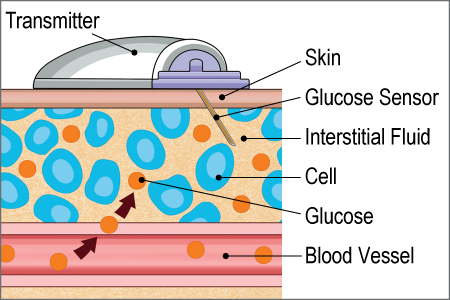
\includegraphics[width=0.5\linewidth]{images/cgm.png}
\caption{Illustration of a CGM sensor.}
\label{fig:cgmsensor}
\end{figure}

State-of-the-art ground truth measurement for plasma glucose is typically ascribed to the Yellow Springs Instrument Glucose Analyzer, but day to day use is handled through handheld Blood Glucose Meters (BGMs). Although accepted as ground truth in many studies, these are far from perfect. The accepted Diabetes Technology Society standard is that a BGM must be accurate to within 15\% at least 95\% of the time, and within 20\% at least 99\% of the time\cite{noauthor_fda_2016}. Many meters do not meet this standard\footnote{A formal study on accuracy is \cite{clarke_evaluating_1987}, more recent informal studies are \cite{scheiner_2016_nodate},\cite{noauthor_are_2017},\cite{edelman_blood_2013}.}. Another popular assessment for BGMs is Clarke Error Grid Analysis (EGA). This is intended to measure clinical accuracy, or the likelihood that a glucose reading will provoke a wrong management decision, and is equally important.

Over the past half decade, CGMs have been working their way into common practice. For immediate management, they give both an instantaneous spot check and an idea of current glucose behaviour, which is very helpful for tailoring action. On top of this, they also give semi-continuous historical data that can be used to get a better idea of glucose response to various environmental variables, which helps significantly for perfecting management. Analysis of the historical record can also lead to a more high definition performance metric.

Although CGMs directly measure interstitial fluid, their accuracy is judged by how close they are to plasma glucose readings. A CGM accuracy will typically be reported as how close the spot checks are to a corresponding BGM reading. Although CGMs also give trend data, performance metrics for this are still being developed within the community. When it comes to clinical accuracy, the basic EGA is often used. However, Continuous Glucose Error Grid Analysis (CG-EGA) is in the late stage of development to judge the clinical accuracy of CGMs based on the wider range of information they provide. 

Blood glucose is the accepted ground truth for all glucose management, because it’s the most reactive metric and already embedded in diabetes care. All other systems, regardless of how they sample glucose, strive to match it. However, continuous monitoring also provides a wealth of other useful information relevant to both diabetics and others.

\section{Sensor Choice}

Among the many commercially available sensors, we used Abbott’s Freestyle Libre. Among other reasons, it was the only one we could use. DexCom is not available in Singapore, and Medtronic only displays to an insulin pump. Being based in Singapore without an insulin pump, Abbott was the only option. It is not strictly speaking a CGM, since it doesn’t broadcast the results, which must be manually checked. Since that’s the only difference, for ease of reference it’s typically included under the umbrella term anyway.

\begin{figure}[ht]
\centering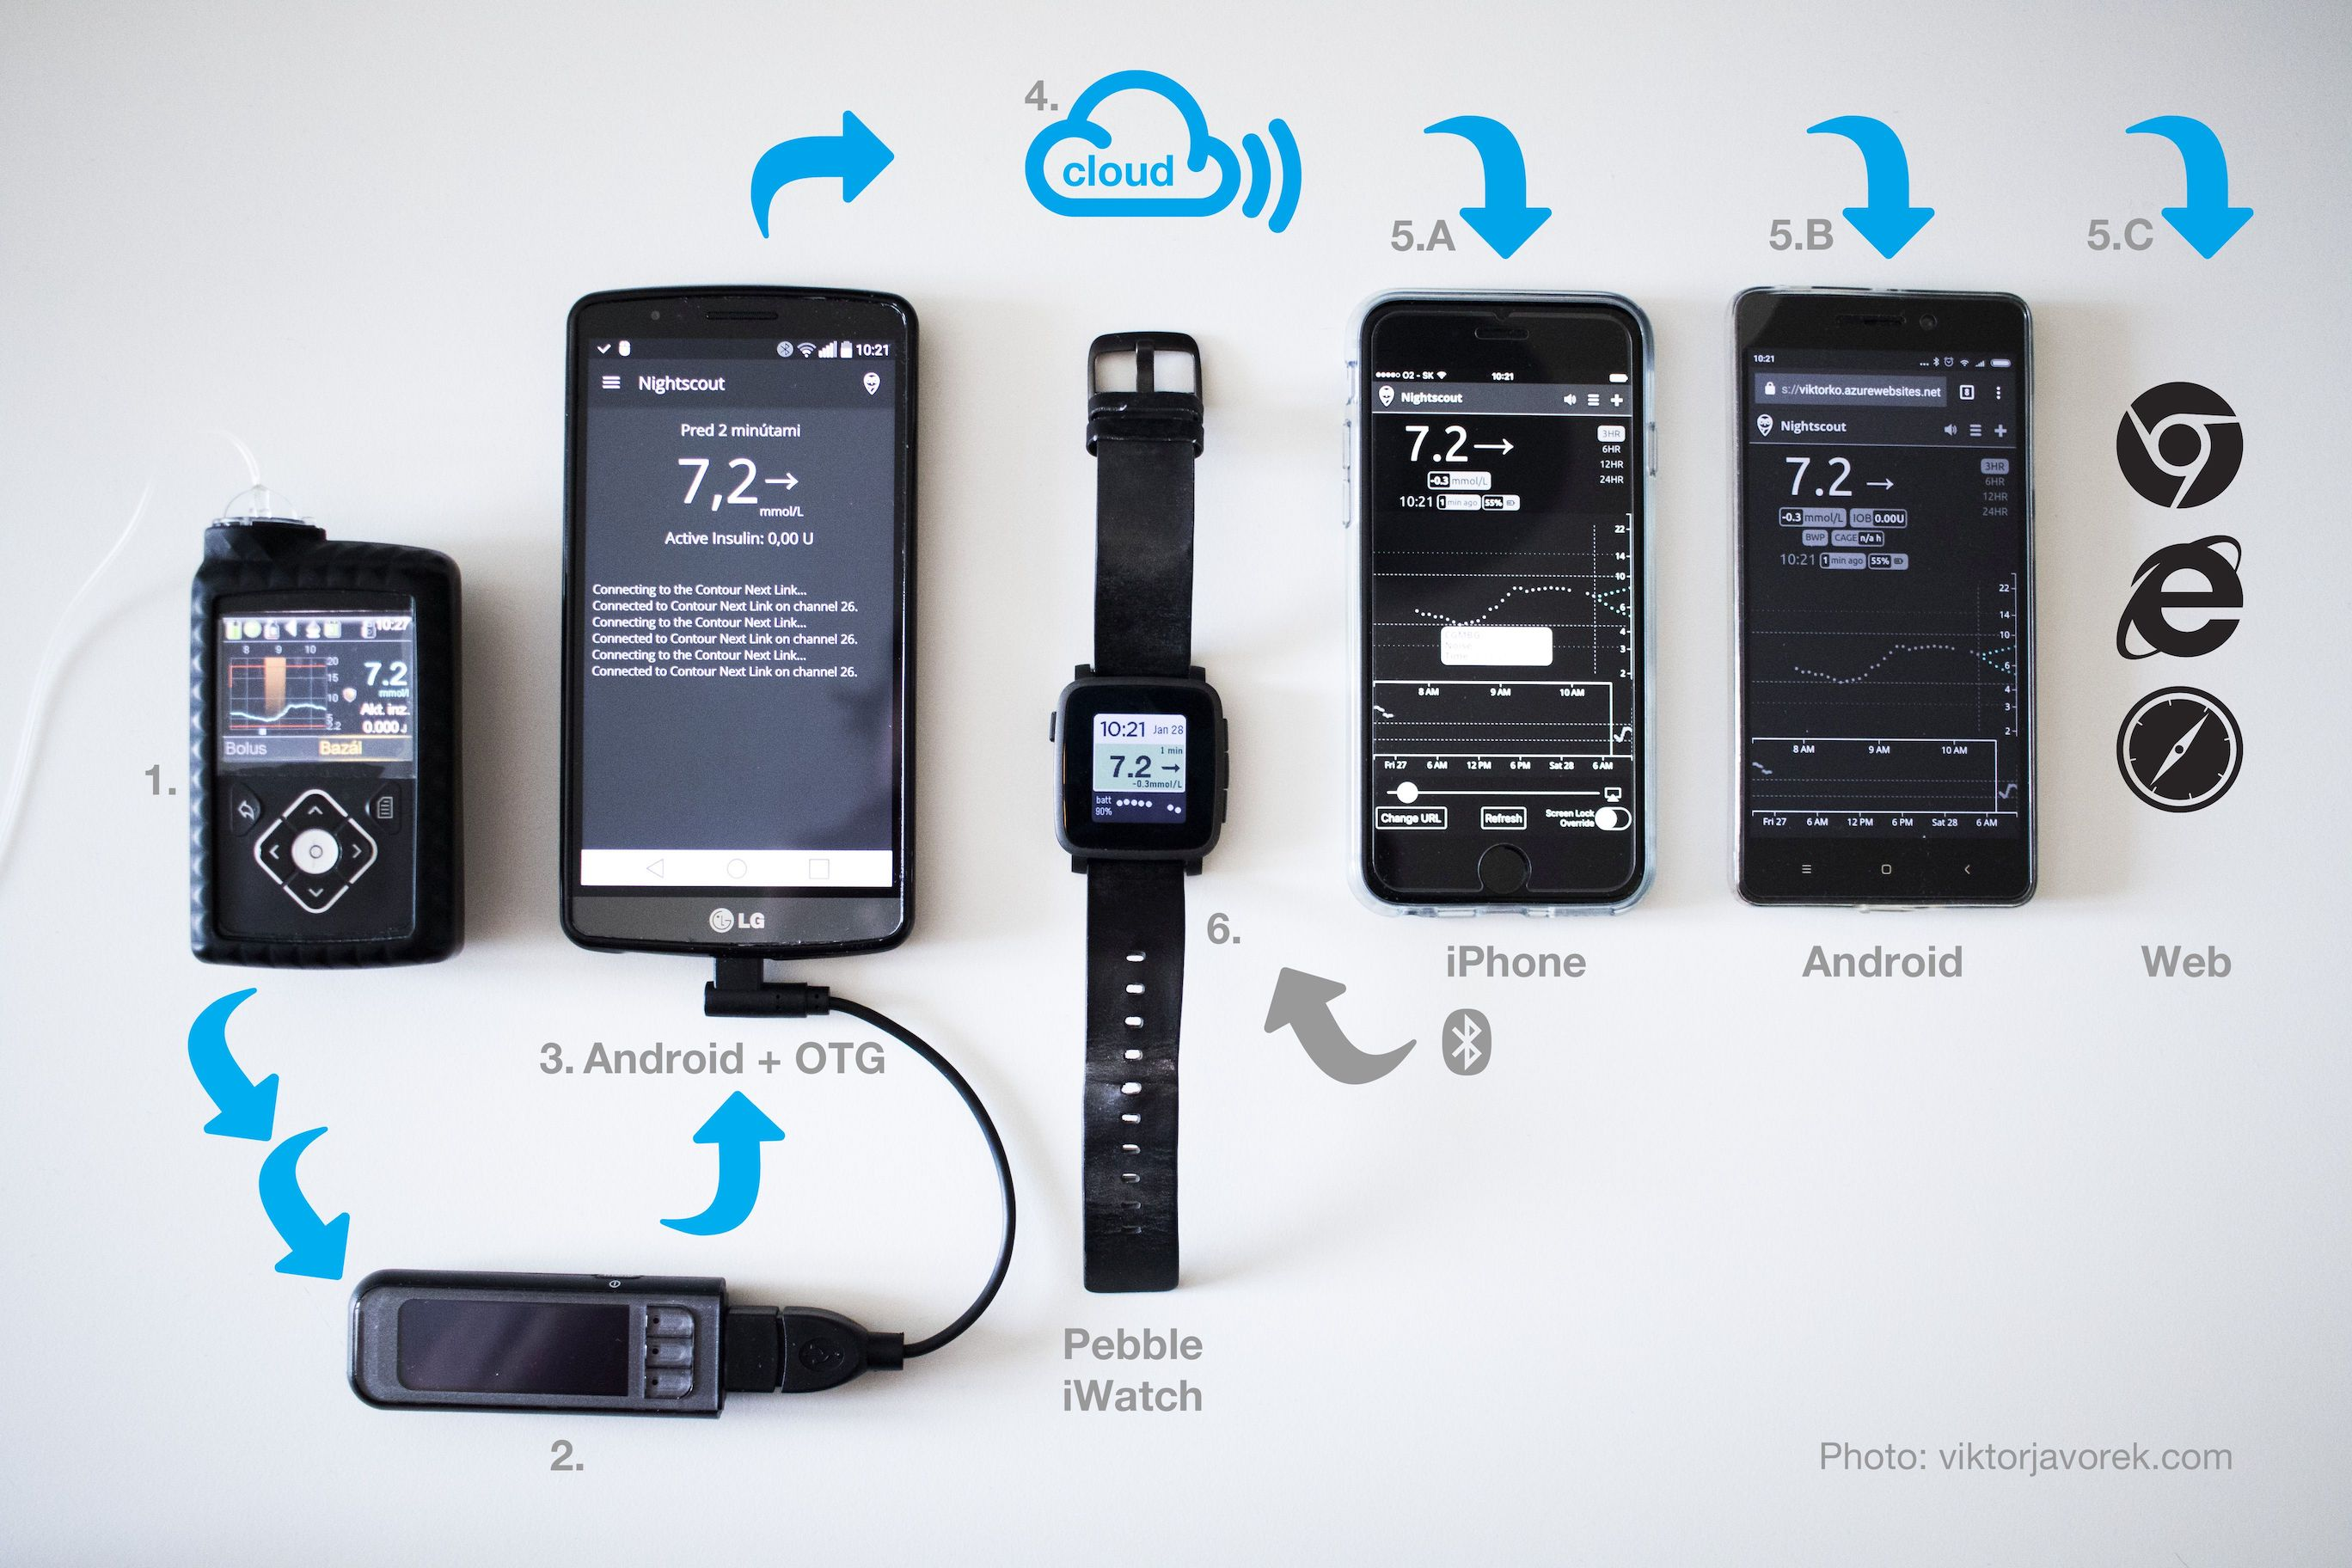
\includegraphics[width=1.0\linewidth]{images/nightscout}
\caption{The Nightscout ecosystem.}
\label{fig:nightscout}
\end{figure}

The Freestyle Libre has several other advantages. It is the cheapest and longest lived sensor available, with appreciable accuracy in all papers. The website is easily the most user-friendly, which is far more beneficial than it sounds. Most relevant to our purposes, it has the largest hacker community already formed. In particular, protocols and proof-of-concept software had been developed for accessing values straight from the sensor, and as we later found out, from the reader. Achieving something similar with DexCom apparently requires soldering together a xDrip device from scratch and online instructions. Data sent from sensor to display can be captured from both DexCom and Medtronic, with an associated GitHub repository. However, it’s more complicated and not intended for personal data analysis, being part of the bigger Nightscout\cite{noauthor_nightscout_nodate} project, which aims to provide a complete framework for managing glucose information.

\section{Freestyle Libre}
The Freestyle Libre CGM\footnote{It must be noted that the FreeStyle Libre is officially classified as a Flash Glucose Monitor (FGM), in that it does not alert the user directly, requiring a scan to do so. However, or the purposes of this report and the framework being built, we will use the terms CGM and FGM independently.} consists of a subcutaneously implanted sensor and hand-held reader. Interstitial fluid readings are taken every 60 seconds, by the method described in detail below. The sensor records these raw values. Scanning the sensor with the reader automatically transmits the stored data through NFC. The reader then processes the raw data and displays a current glucose value, 8hr historical trend line, and an arrow indicating trend direction.

Studies have shown \cite{abbott_real-world_nodate} that using continuous glucose monitors (the Freestyle Libre in particular) have resulted in a 16\%reduction in HbA1c levels, as well as significantly lower occurrence and duration of hypoglycemic episodes.
\chapter{Technical Analysis}

\section{Event Analysis and Review}

The FreeStyle Libre sensor takes readings every 60 seconds, but it does not retain all of these, for what we presume are storage limitations. Instead, it keeps half an hour of high definition data (30 values separated by 60 seconds) and an additional 7.5 hrs of coarse 15 minute data (45 values separated 15 min), disregarding the rest. The sensor also contains a power source, for both the electronics and the measurement mechanism, and a thermometer. When scanned, the sensor provides the stored data (30min fine, 7.5hr coarse), associated internal time and uncalibrated temperature information. This information was gained during data analysis, as discussed later on in section x.

The sensor provides a series of raw, unsmoothed datapoints at a lag from ground truth, which the reader aims to transform into clinically appropriate information. Their precise algorithm is appropriately a trade secret, but provides transformed historical data, point estimate, and trend. Sometimes it will refuse to display any data, typically if glucose levels are changing very rapidly. Since the company provided accuracy study uses industry-standard Yellow Springs Instrument levels as ground truth, the provided data can safely be assumed to be intended to represent venous blood glucose. Their user manual also provides a chart for interpreting the glucose trend arrow, as shown in Figure~\ref{fig:arrows}\footnote{from the FreeStyle Libre manual supplied with the sensor.}. We found that the reader point estimate provides greater mathematical accuracy to blood glucose than the associated raw sensor value. The historical trend line is displayed in too low a resolution for much accuracy discussion, but as discussed later, more data can be gained. The trend arrow will be discussed more in depth in future. Of course, clinical accuracy must also be considered.

\begin{figure}[ht]
\centering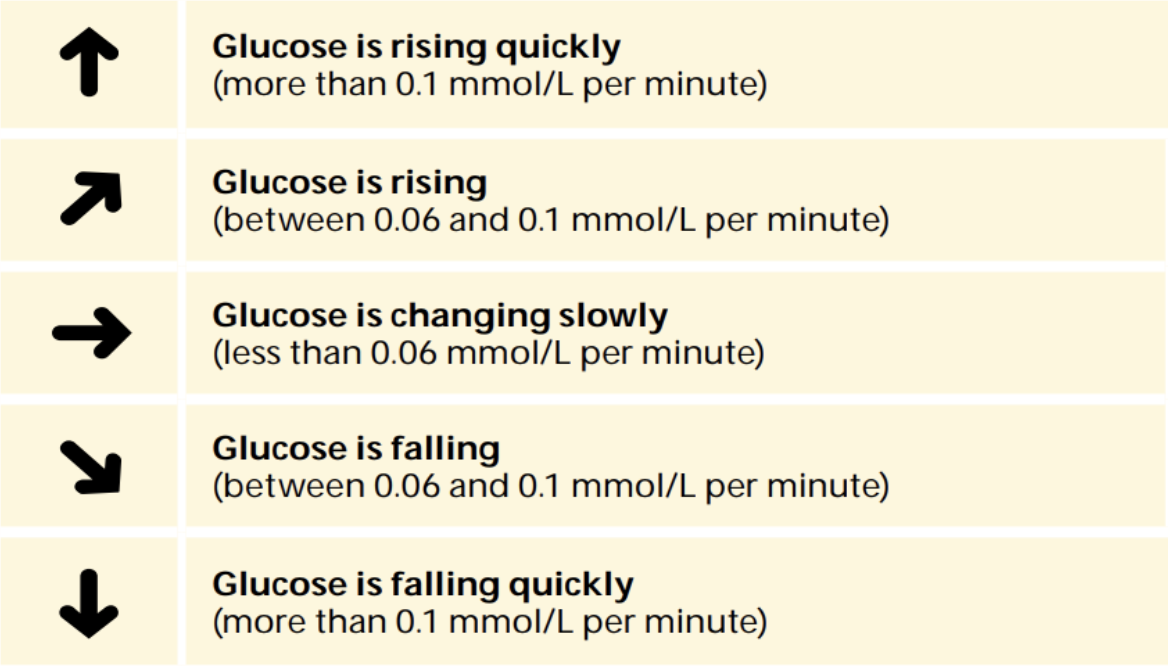
\includegraphics[width=1.0\linewidth]{images/arrows.png}
\caption{Conditions where arrows are displayed.}
\label{fig:arrows}
\end{figure}

As well as processing and displaying the raw data, the reader provides several extra capabilities. It allows users to set date, time and target glucose range. With each scan, it also allows the user to add flags to record extra events such as insulin, food, medication and exercise. Flags for other events can be added using the software. Historical records can be viewed as well as limited analytics such as weekly averages, time in range, and typical daily trend. The reader can also act as an independent blood glucose or ketone meter.  

\section{Sensor Chemistry}

The technology underlying most commercially available continuous glucose monitors is the same. They are inserted subcutaneously, typically into the arm or stomach. They consist of an implanted, flexible catheter attached to the external plastic shell, which is typically attached to the skin with adhesive. The catheter acts as an amperometric biosensor and takes a raw measurement of interstitial glucose. The external hardware provides power, keeps time, and records the measurements, and is sometimes attached to an optional transmitter. Currently, there are three main commercial brands; DexCom, Medtronic, and FreeStyle.

\subsection{Amperometric Glucose Biosensors}

An amperometric glucose biosensor uses redox electrodes to create and measure a current proportional to interstitial glucose concentration. From the current, they can closely estimate the actual glucose concentration. If there’s too much noise for the current and concentration to have a constant ratio, the device will require regular recalibration by matching with blood glucose tests. Since most CGMs aim to eliminate the need for BGMs, manufactures aim to reduce noise, while maintaining sensor lifespan and comfort.

\begin{figure}[ht]
\centering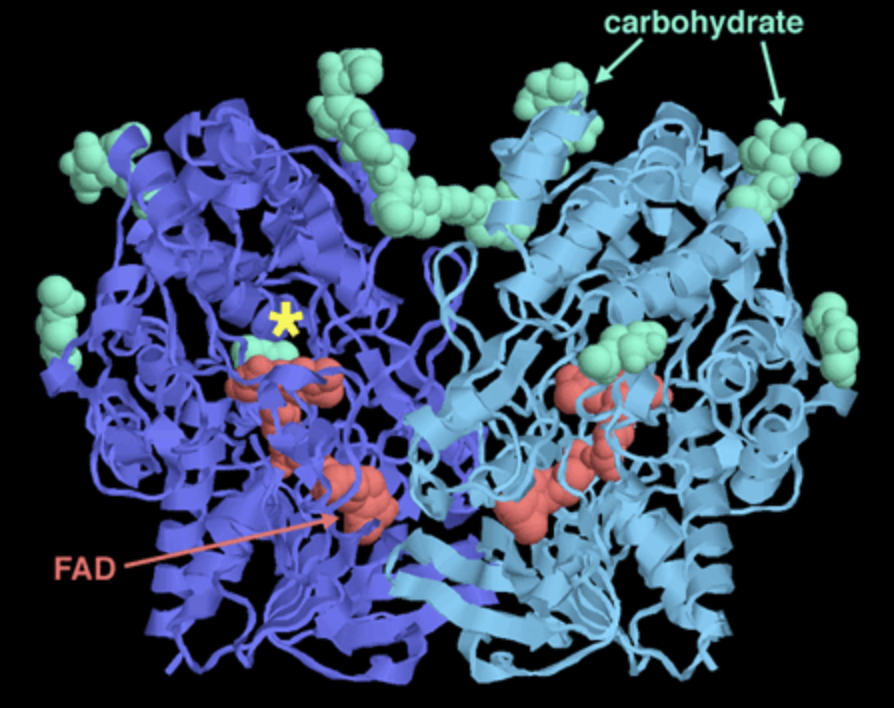
\includegraphics[width=1.0\linewidth]{images/mom.png}
\caption{Location of flavin adenine dinucleotide (FAD) co-factor in glucose oxidase.}
\label{fig:mom}
\end{figure}

In order to produce the proportional current, an amperometric biosensor electro-oxidizes glucose with glucose oxidase as shown in Equation~\ref{eq:one}, then measures the current provided when re-oxidizing the reduced glucose oxidase. It is difficult to directly oxidize the glucose oxidase FAD co-factor, since it’s buried deep within the molecule (Figure~\ref{fig:mom}), a mediator is usually used. This creates a three step system: oxidize glucose with glucose oxidase, react with the mediator, then oxidize the reduced mediator. At each of these steps, the concentration of the products remains proportional to the concentration of glucose. At the last step, the electro-oxidation of the mediator, the current produced will also be proportional. The speed of electron movement will be proportional to the reaction rate, which will be proportional to the reactant (reduced mediator) concentration\cite{noauthor_amperometric_nodate}. This provides an acceptable raw representation for interstitial fluid glucose concentration. Anything that interferes with any of these proportionalities creates noise.

Most often, oxygen is used for the mediator. This results in the chain of reactions shown in Equations~\ref{eq:two} and \ref{eq:three}. Oxygen is a useful mediator, because instead of needing to be immobilized in on the electrode, it can be taken in vivo. However, the reactions need a higher ratio of oxygen to glucose that is found in interstitial fluid to be successful. To overcome this, both Dexcom and Medtronic have developed complicated membranes that only allow the desired ratios in - remaining, of course, in proportion to the global body glucose\cite{noauthor_mary_nodate}. However, this introduces more noise. The heavy design requirements for the membrane also means that they can’t adapt it as well to control other noise-inducing factors. This contributes to both those systems requiring twice-daily calibration.

\begin{equation} \label{eq:one}
FAD-GO_x + glucose \rightarrow FADH_2-GO_x + gluconolactone
\end{equation}

Reduction half-equation: $FAD-GO_x + 2H_+ + 2e+-  FADH_2-GO_x$\\ 
Oxidation half-equation: $glucose \rightarrow gluconolactone + 2H_+ + 2e_- $

\begin{equation} \label{eq:two}
FADH_2 - GO_x + O_2 \rightarrow H_2O_2 + FAD-GO_x 
\end{equation}

Reduction half-equation: $O_2 + 2H_+ + 2e_- \rightarrow H_2O_2$ \\
Oxidation half-equation: $FADH_2 \rightarrow FAD-GO_x + 2H_+ + 2e_-$ 

\begin{equation} \label{eq:three}
 H_2O_2 \rightarrow O_2 + 2H_+ + 2e_- 
\end{equation}

Abbott overcame this issue with their trademarked  Wired Enzyme technology\cite{noauthor_sensor_nodate}. This uses immobilized osmium complexes as their mediator, resulting in the reactions shown in Equation~\ref{eq:four}. This has several benefits. It avoids involving extra unknown factors into the equation by removing the need to use internal oxygen and by oxidizing the glucose oxidase in place, instead of in solution. Most usefully, re-oxidizing the osmium requires a much lower voltage than doing so for the oxygen. This avoids interference from other substances, like uric acid or medical acetaminophen\cite{noauthor_mary_nodate}. Overall, the Wired Enzyme decreases noise enough that it need only be calibrated in the factory, since the current to glucose concentration ratio stays constant\cite{hoss_feasibility_2014}. On the other hand, it means that Abbott devices have a clear expiration date, since they can’t keep working once they run out of osmium.

\begin{equation} \label{eq:four}
FADH_2 - GO_x + 2Os_{3+} \rightarrow  2Os_{2+} + FAD-GO_x + 2H_+ 
\end{equation}
Reduction half-equation: $2Os_{3+} + 2e_- \rightarrow 2Os_{2+}$\\ 
Oxidation half-equation: $FADH_2 \rightarrow FAD-GO_x + 2H_+ + 2e_-$ 

Other factors also confound accuracy. Regardless of what mediator a sensor uses, it has to resolve biofouling. Tissue response to a foreign body injection can mean that local glucose stops accurately representing global glucose. Companies minimize this with increasingly biocompatible materials. Another problem which is yet to be properly solved is tissue inflammation upon injection. This typically means that initial results will be less accurate, getting more so as the inflammation goes down.

One environmental variable that hasn’t been properly addressed is temperature. All amperometric biosensors rely on enzyme reactions, which vary heavily with temperature\cite{noauthor_accuracy_nodate}. Enzyme activity increases alongside temperature, which carries over throughout the process and hence to the reported glucose values. No mention can be found of how any CGM controls for this within the sensor hardware, and it’s difficult to imagine how they could. 

CGM sensors record interstitial fluid glucose by using an amperometric biosensor to measure a current that’s directly proportional to glucose concentration. In order to make sure that the proportionality remains, companies have put a lot of work into minimizing chemical and biological interference. 


\chapter{Development}

Below is the process of developing a glucose monitoring app using the FreeStyle Libre FGM sensor, which involved reverse engineering the protocol of the Libre, and developing a system for calibration and conversion of raw sensor and temperature values into readings. The application also features speed improvements over current state of the art, and is designed to be open source to function as a platform for building predictive and analytics tools based on such data, in addition to data aggregation.

\section{Architecture}

\begin{figure}[ht]
\centering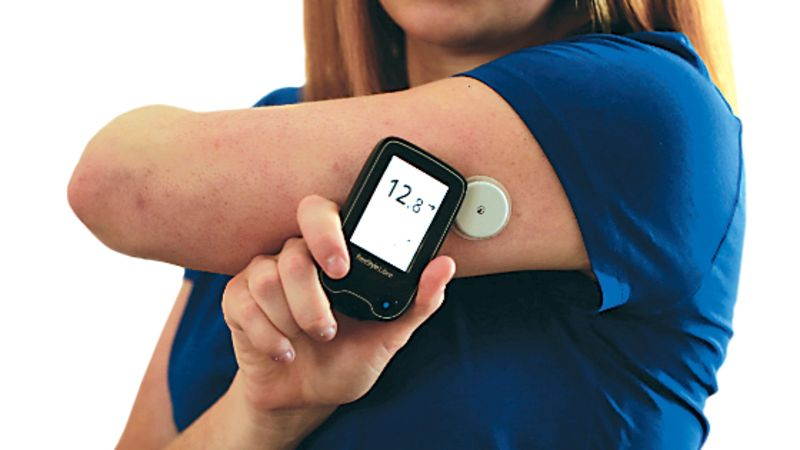
\includegraphics[width=0.4\linewidth]{images/libre1}
\caption{Freestyle Libre sensor and reader in use\cite{noauthor_how_2017}.}
\label{fig:libre1}
\end{figure}

The sensor used in the Freestyle Libre (hereafter referred to as \textit{the sensor} for brevity) is described in multiple patents\cite{noauthor_patents_nodate}, which outline the design and electrochemical composition of the system. Figure~\ref{fig:libre1} shows the scale of the sensor and the reader. Most relevant here are the ones that describe the sensor chemistry as well as notes on the encoding patterns. The chemical method being used\cite{say_electrochemical_2000} is described to vary linearly with temperature as well as the concentration of interstitial fluid glucose. The raw values thus extracted from the electrode on the sensor are then stored in a processing unit on the sensor, as underlined by the patent. 

\begin{figure}[ht]
\centering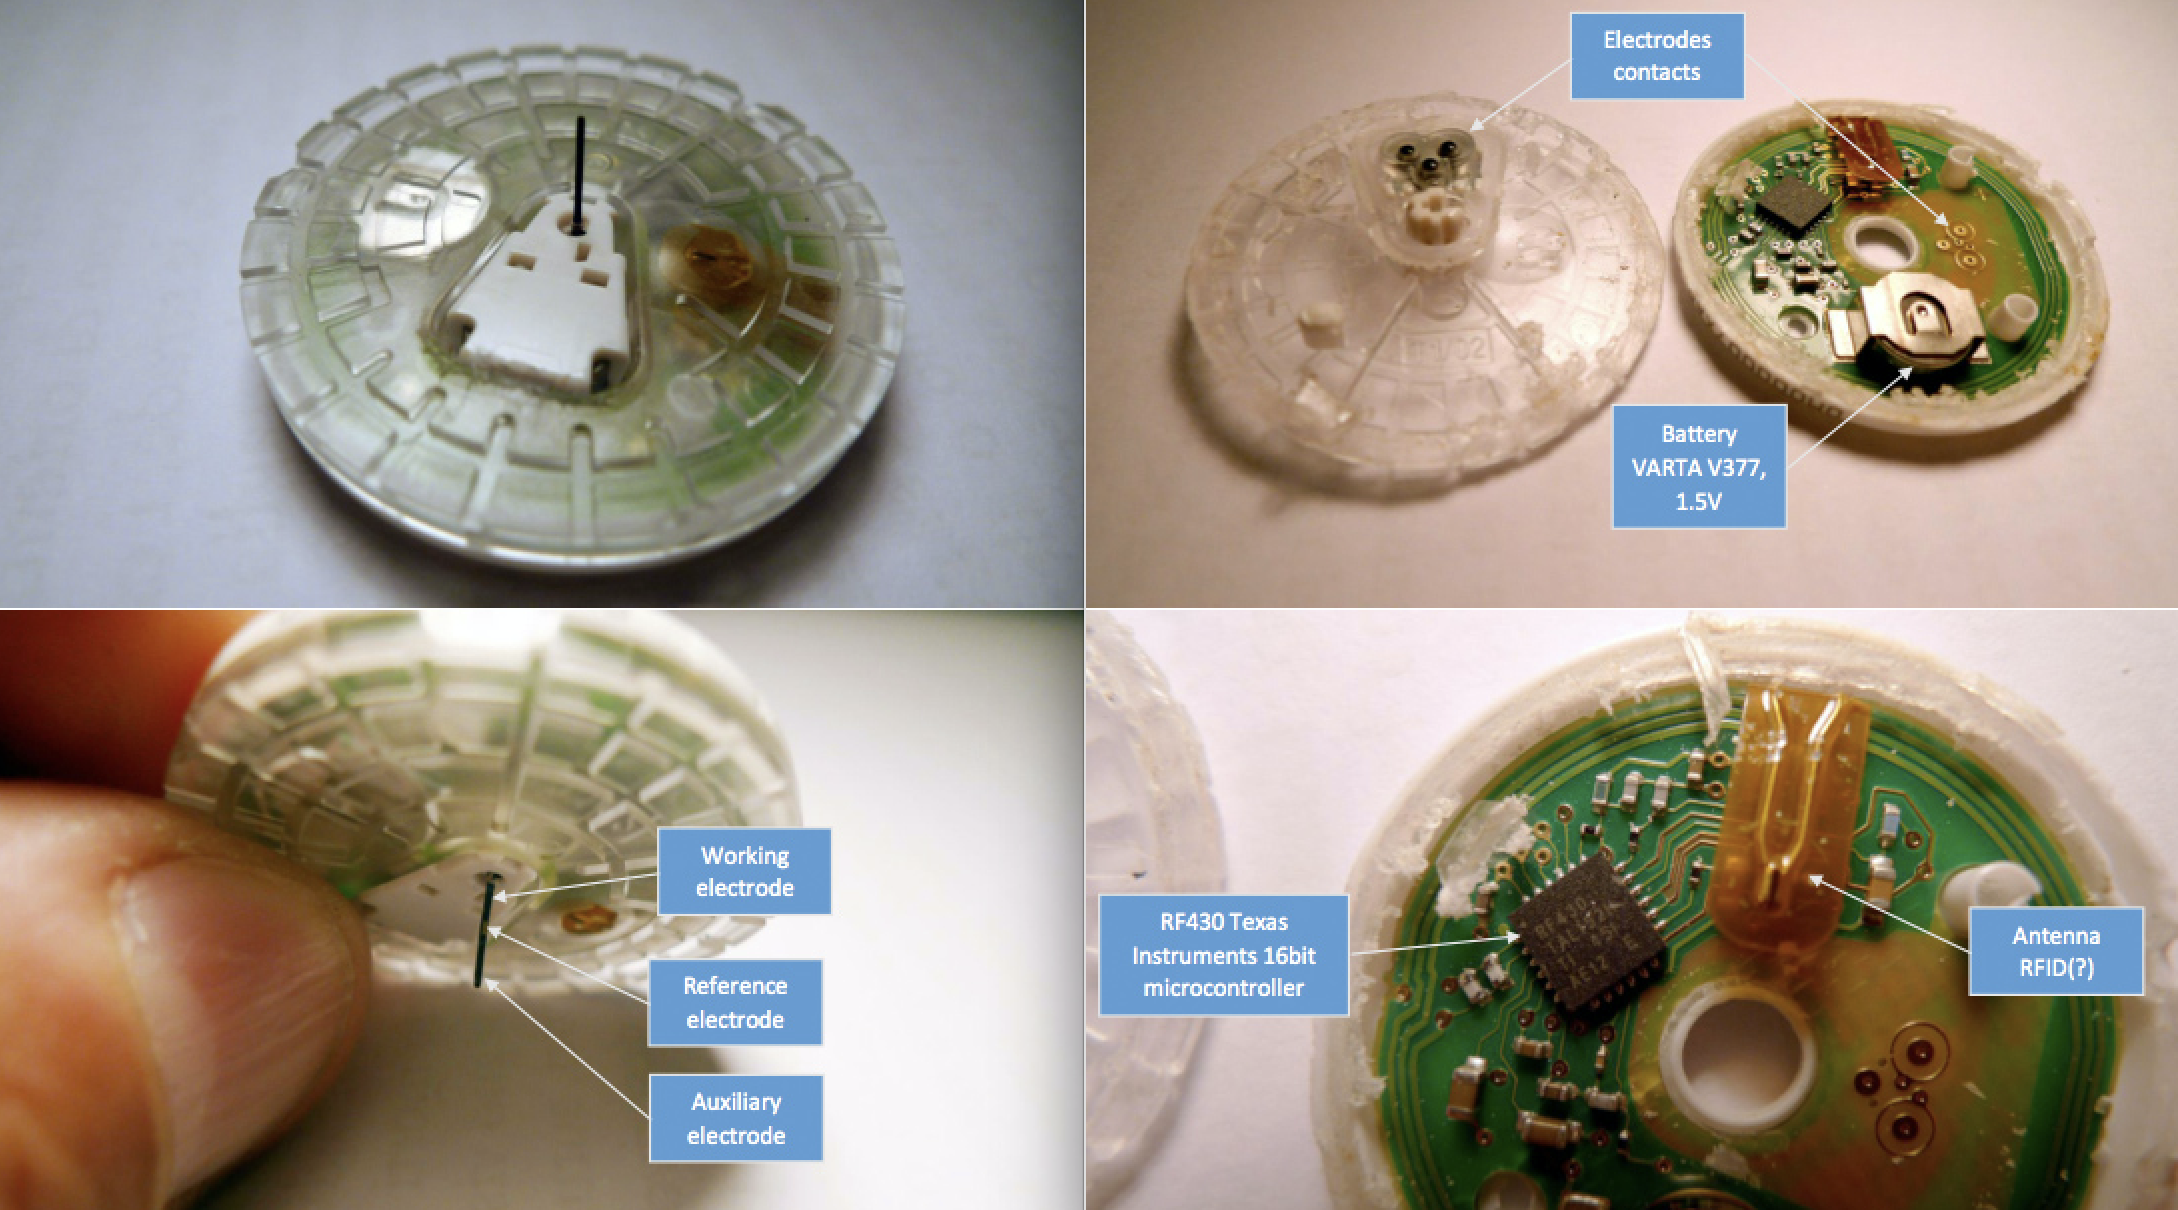
\includegraphics[width=1.0\linewidth]{images/libre4}
\caption{External and internal components of the sensor\cite{ilka_freestyle_2014}.}
\label{fig:libre2}
\end{figure}

A teardown view of the sensor is presented in Figure~\ref{fig:libre2}, where the processor being used as well as the internal components can be identified. Glucose measurement, as previously discussed, is taken via an amperometric biosensor which is primarily encapsulated within the flexible needle. The sensor apparatus also contains a thermocouple tape \cite{noauthor_thermocouple_1971} which reacts linearly(within thresholds underlined in the patent) to temperature. Single-point and dual-point calibration systems are mentioned, by the use of which the raw sensor glucose information can be calibrated to the internal temperature of the sensor. The only visible temperature sensor\footnote{It must be noted that the processor carried an on-board temperature sensor. However, it is unknown how this is used.} is on-board the sensor body, taped to the plastic housing on the side of the user's skin. This leads us to believe that a single-point calibration is being used, which will be confirmed later.

The processor (from the product number) is an  RF430FRL152H\cite{noauthor_rf430frl152h_nodate}
\footnote{a member of the MSP430\cite{noauthor_16-bit_nodate} family of low-power microcontrollers by Texas Instruments}, which is used to read and store raw values from the sensor, and communicate them over a Near-Field Communication(NFC)\cite{noauthor_near-field_2017} protocol to the reader apparatus. Unfortunately there are no accessible debugging points on the circuit board, so most of the work will need to be done through the wireless protocol on board.

An on-board battery powers the sensor during operation, however, the patent does not describe any mechanisms for calibrating the voltage drift from the battery provided DC voltage. This was surprising, and leaves potential room for additional work on whether this is a factor.

\begin{figure}[ht]
\centering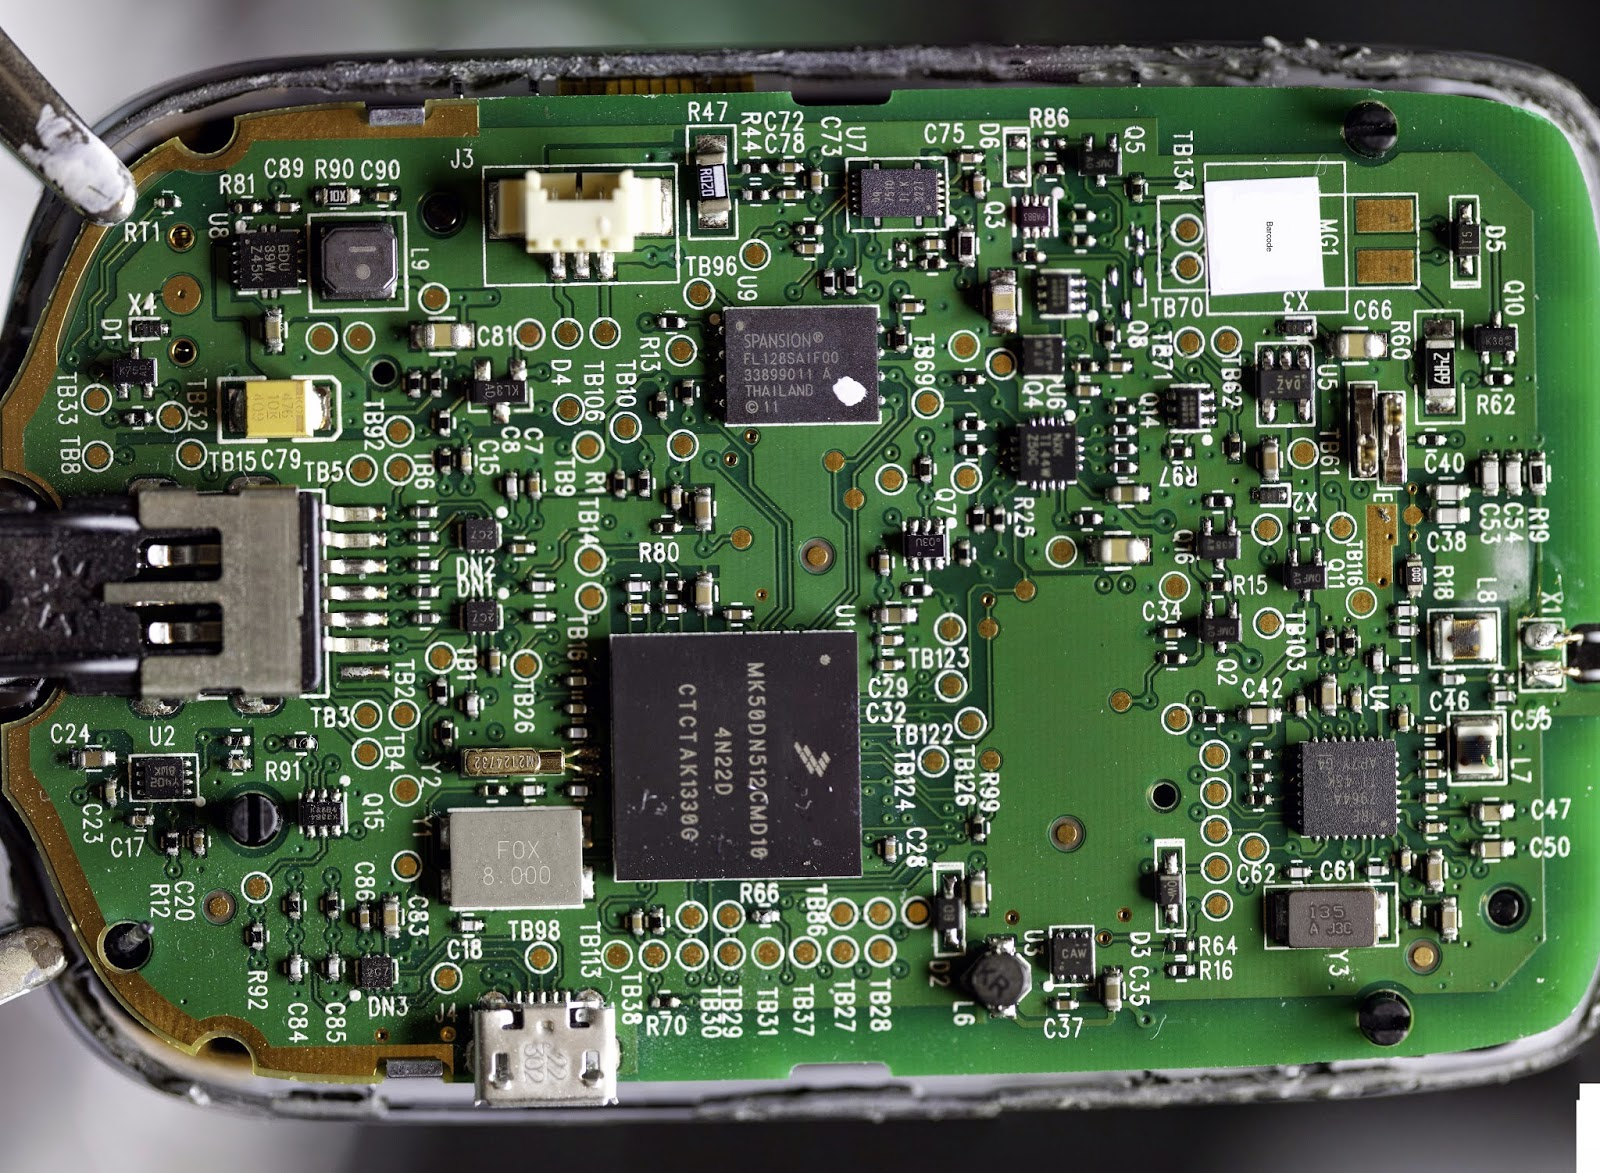
\includegraphics[width=1.0\linewidth]{images/libre5}
\caption{Internal PCB of the reader\cite{noauthor_type_nodate}.}
\label{fig:libre3}
\end{figure}

The reader apparatus (Figure~\ref{fig:libre3}) is unsurprisingly complex, as it incorporates the mechanism for reading and processing sensor data, USB interfacing components as well as a blood-glucose test strip reader. The internals are well weatherproofed, and the construction is remarkably robust. The existence of a number of test pads (possibly for in-factory calibration and quality control) as well as an unexposed connector leave future avenues for extracting information from the reader.

\section{Communication Protocol Analysis}

The datasheet\cite{noauthor_rf430frl152h_nodate} for the on-board processor of the sensor describes use of the ISO 15692 protocol\cite{noauthor_iso/iec_2017}, and reading the information using an NFC reader application on an Android phone confirms it conforms to the Nfc-V\cite{noauthor_nfcv_nodate} standard, which is a distance-limiting version of the ISO protocol. This limits the effective use of a reader apparatus to a few centimeters\cite{noauthor_nfc_nodate}, but also means that all new Android smartphones with NFC technology will be able to read the sensor with the same protocol. The manufacturer is listed as Texas Instruments, with 1952 bytes of memory being transmitted on a full read. Armed with this information, we can proceed.

\subsection{Related Work}

A number of projects have attempted to use the Freestyle Libre as a Continuous Glucose Monitor. There have also been a number of attempts to reverse engineer the protocol being used and to extract the values therein. The most popular (with about 50,000 downloads) of which is the Android application Glimp\cite{software_glimp_2017}, which 	reads the FreeStyle Libre sensor and claims to "calibrate" the sensor using Blood Glucose readings independently provided by the user. Unfortunately, this project is not open source, and the available open source offerings do not go further than reading raw glucose values without calibration or temperature data, and suffer from long read-times (exceeding 2 seconds) for the sensor. Users have also reported that the measurements thus provided are often wrong, and often dangerous - in fact, as one particular analysis shows, the calibration methods used lead to often fatal predictions for users\cite{v_libre_nodate}. The closest project that could be found was the FreeStyleLibre-NFC-Reader\cite{bautista_freestylelibre-nfc-reader:_2017} project, which displayed the most recently recorded sensor value\footnote{Small caveat being that the code was largely uncommented and labeled in Spanish.}. Looking at available solutions for working with the FreeStyle Libre system indicated the dire need for open source projects that aim to improve on intelligent reporting as well as detailed documentation on internal working.

The accompanying Wiki article was useful in providing the following information:

\begin{enumerate}
\item The glucose data being recorded on the sensor is split into 16 measurements spaced one minute apart and 32 measurements spaced 15 minutes apart.
\item A circular array is used for writing the data (presumably to minimize rewrites to memory), and the next write position is recorded in the hex before the two arrays.
\item The numbers are encoded in Little Endian Binary\cite{noauthor_endianness_2017}.
\end{enumerate}

However, the author states that his analysis is purely experimental, and that it fails on a sensor that is in use for more than 10 days (the labeled use period of the sensor is 14 days). However, this provides a suitable starting point if we proceed with caution.

\section{HEX Analysis}

\begin{figure}[ht]
\centering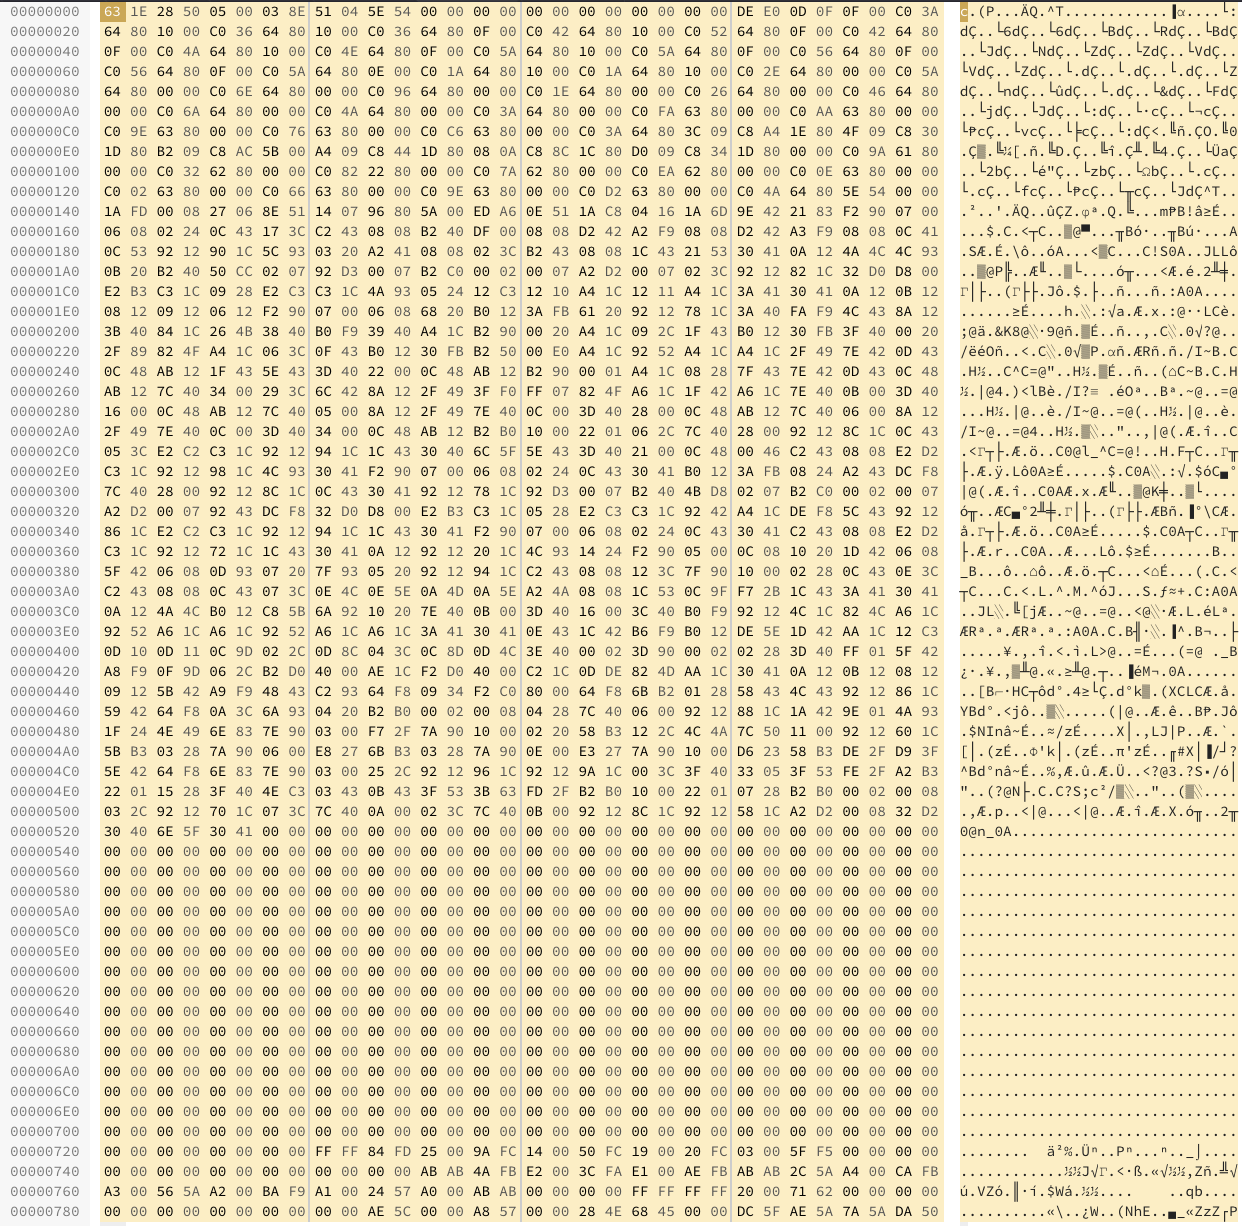
\includegraphics[width=0.5\linewidth]{images/hexdump.png}
\caption{Full hexadecimal and ASCII character dump of sensor tag memory.}
\label{fig:hexdump}
\end{figure}

Visual analysis of the tag memory indicates that a large amount of whitespace remains (Figure~\ref{fig:hexdump}), and comparing to sensor read times for the full tag as opposed to existing solutions (Glimp, Liapp, etc), we can predict that reading only the required bits of the sensor will let us speed up this process considerably.

A python program\footnote{processrawNFC.py in source code} to process the resulting XML and convert it to an addressable array of hex values enables analysis. Considering a differential of consecutive sensor data dumps, we can see the bytes that differ. 

\begin{figure}[ht]
\centering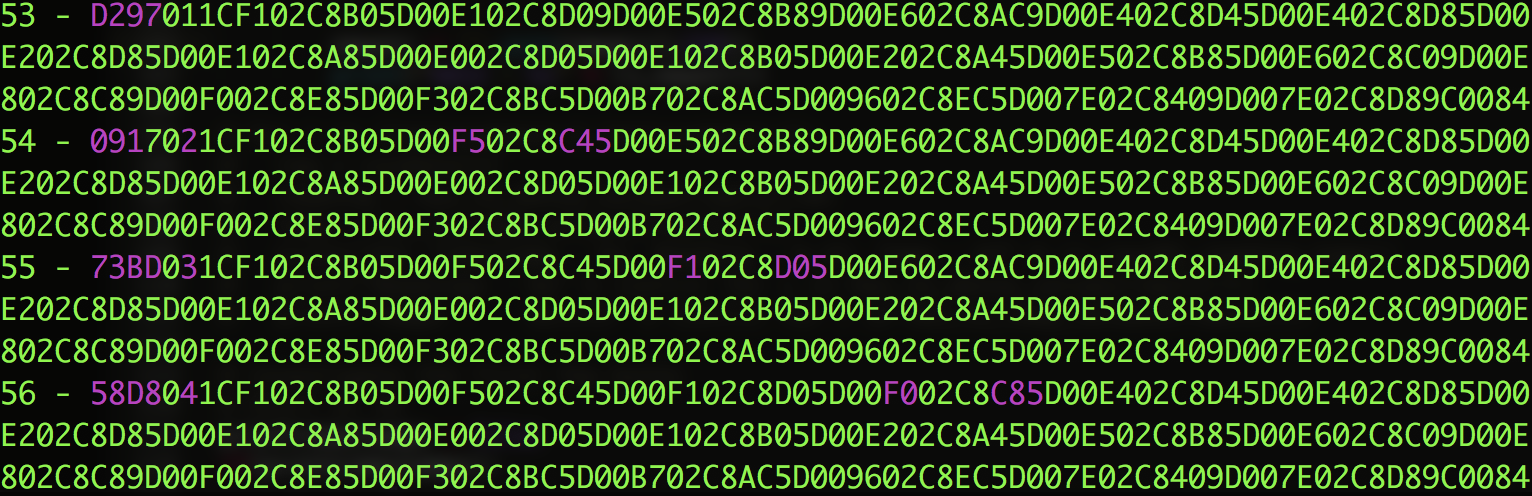
\includegraphics[width=1.0\linewidth]{images/diff.png}
\caption{Differential of sensor hex dumps, with differing bits highlighted in pink.}
\label{fig:diff}
\end{figure}

Figure~\ref{fig:diff} shows hex dumps collected approximately spaces 1 minute apart, which confirm and locate the spots where readings are written. From here, we can take consecutive readings to determine the location of each individual reading, until the write array returns to the same location.

Once this was completed, research suggested that the written values were a combination of flags, raw glucose data and temperature data. What remained was to separate them. This proved simple - removing the sensor from it's position in the body (after insertion and calibration by the reader) provided consistent glucose readings of -2.1. Given that this was a constant factor, binary analysis revealed that the glucose values were encoded in the lower 3 bytes of the reading, and could be deciphered using Equation \ref{eq:glucoseeq}.

\begin{equation} \label{eq:glucoseeq}
V_{glucose} = \frac{V_{raw}\;\mathrm{\&\; 0x000FFF}}{6}-37 
\end{equation}

Next, the glucose information was calibrated using previously collected raw glucose data from Glimp\cite{software_glimp_2017} which could be matched with processed data extracted from the reader using protocols defined in the open source project Glucometer-protocols\cite{petteno_glucometer-protocols:_2017}. The raw and calibrated data seemed to possess mostly a first order aka linear correlation across sensors (Figure~\ref{fig:corr}, and the value of intercept and slope were used to further adjust raw data collected.

\begin{figure}[ht]
\centering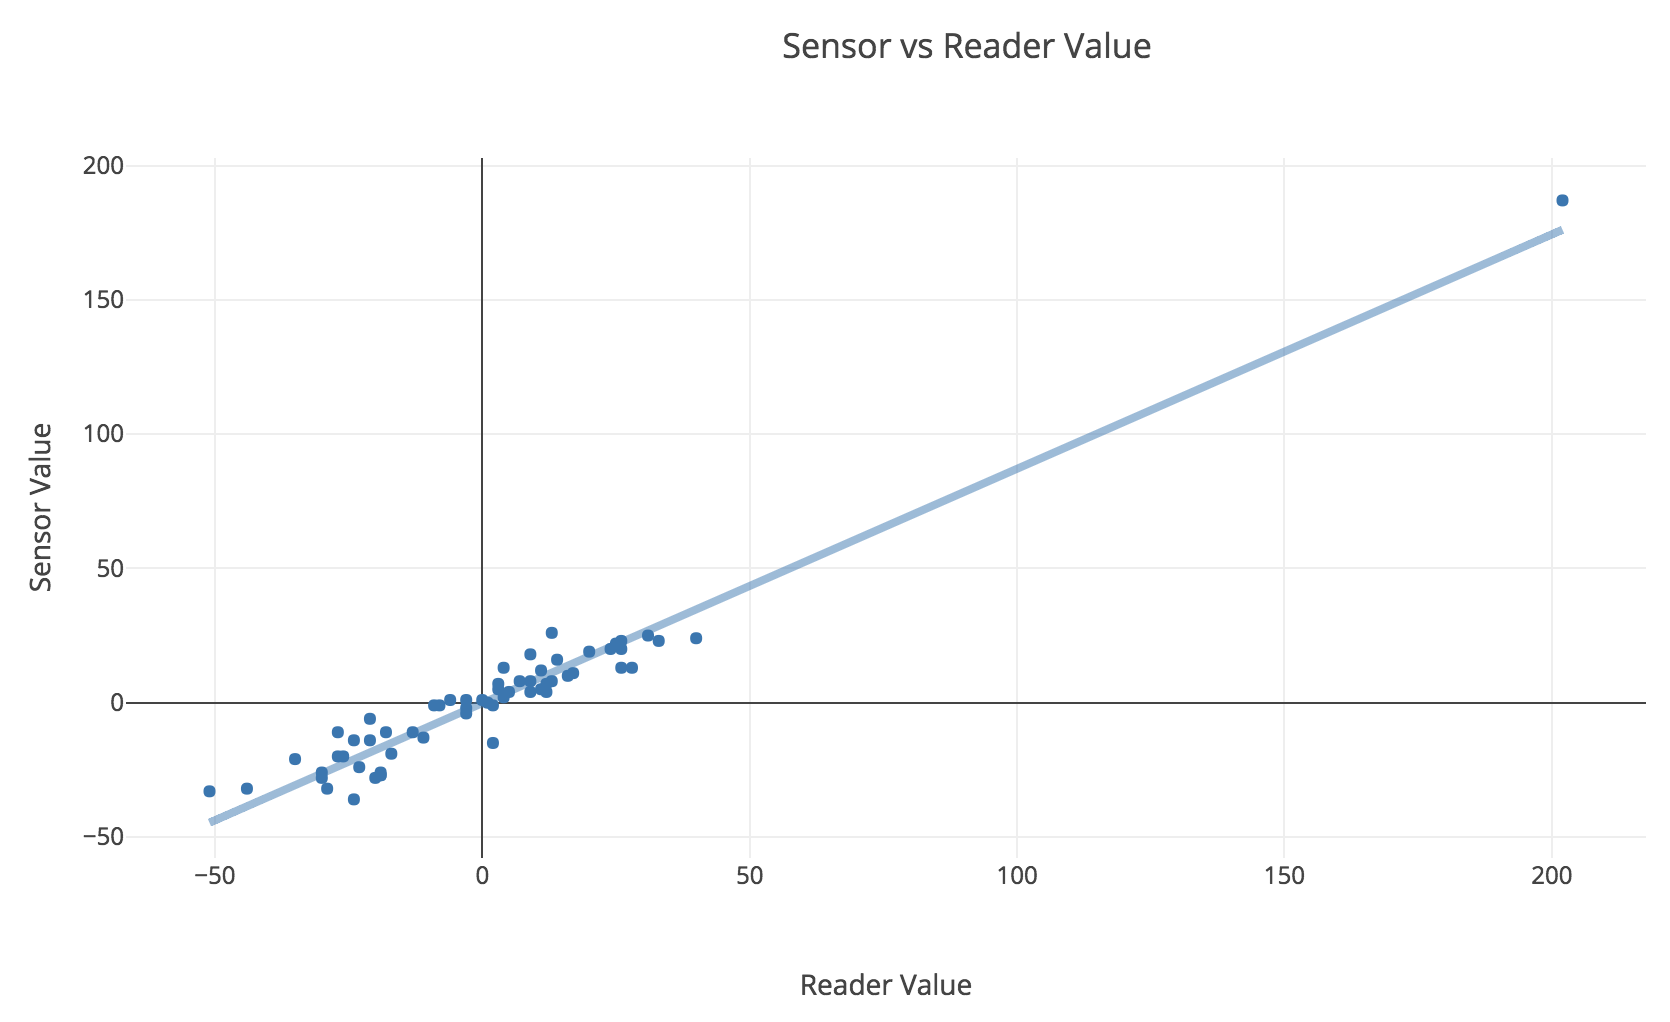
\includegraphics[width=1.0\linewidth]{images/sensorvsreader.png}
\caption{Graph of raw sensor vs processed reader glucose values.}
\label{fig:corr}
\end{figure}

Next was the process of extracting and calibrating temperature sensor information. A simple experimental setup using a multimeter thermocouple taped to the sensor (which was placed closest to the external thermocouple in Figure~\ref{fig:libre2}), following which the apparatus was placed in multiple temperature systems, the average of which was calculated. Once again, the datasheet~\cite{noauthor_rf430frl152h_nodate} was helpful in expecting a linear correlation between temperature and raw values, so a slope, intercept, and a bitmask for the flags was all that was required.

Graphing the resulting data revealed certain flags being turned on and off, which combined with the knowledge that a flag change could be removed with a power of 2, resulted in the bitmask being set at \textbf{0x2FFF}, applied to the upper three bytes of the six-byte reading extracted (the same value can be applied to the entire reading, left shifted). The experimental setup and bitmask evaluation can be found in Figure~\ref{fig:tempcalsetup}.

\begin{figure}[ht]
\centering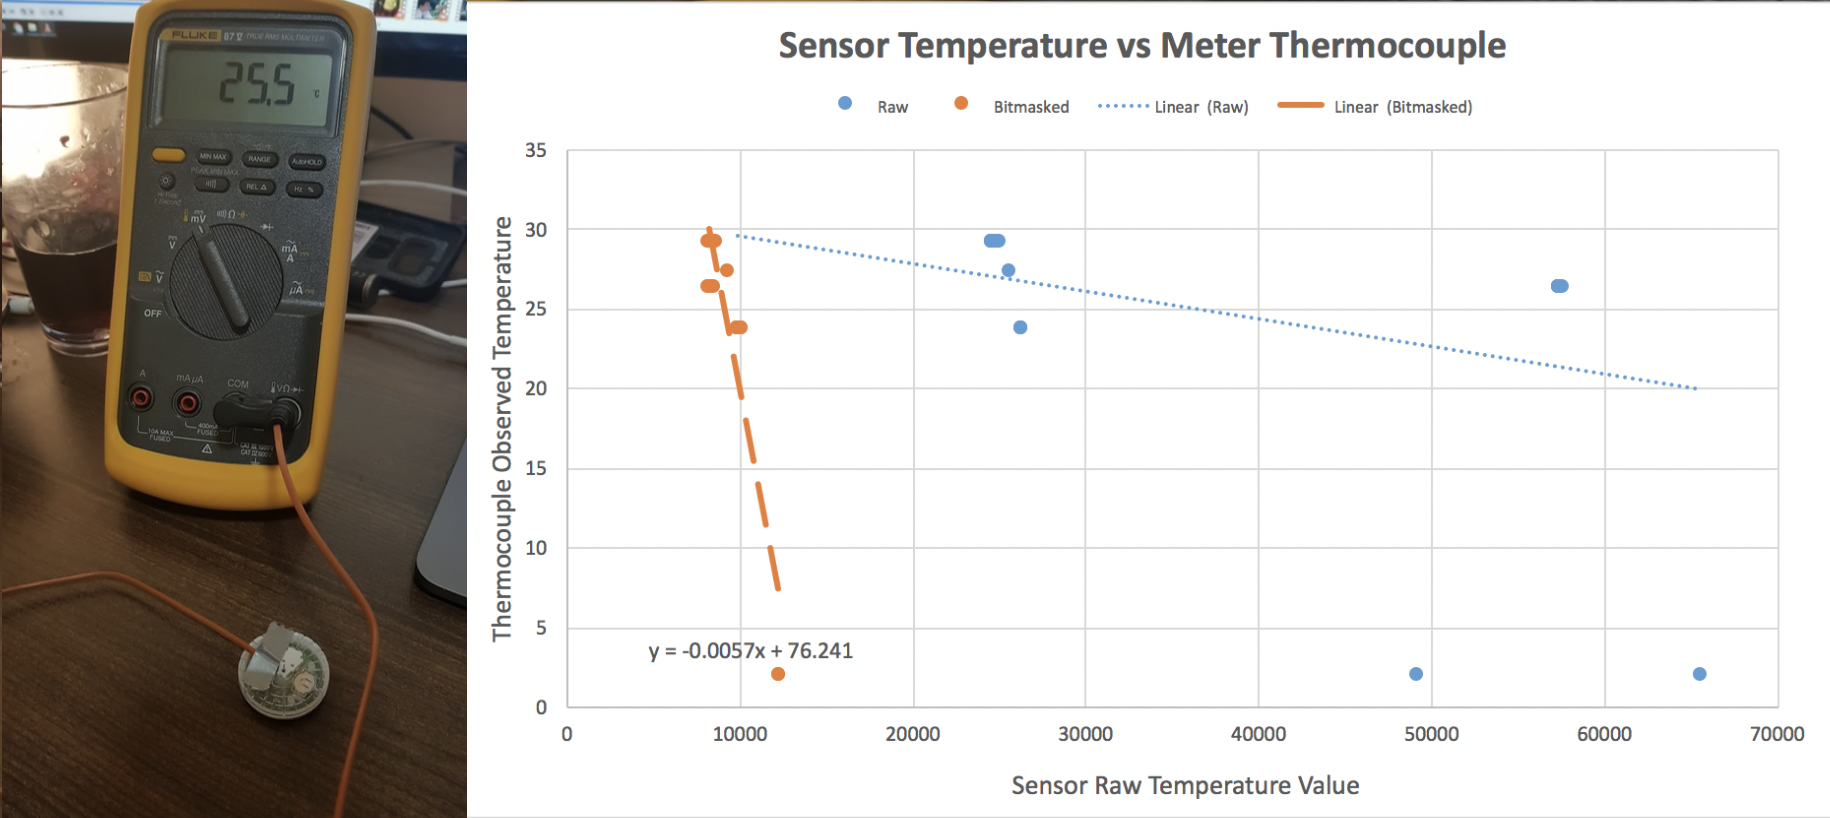
\includegraphics[width=1.0\linewidth]{images/tempcalsetup.png}
\caption{Experimental Setup and bitmasking results of Temperature Calibration.}
\label{fig:tempcalsetup}
\end{figure}

Next, the setup was placed in more accurate ovens that provided better temperature references. In each case, the entire apparatus was placed for a period of 16 minutes. This was due to the uncertainty of the sensor's reading within a minute. Once all previous short term memory had been overwritten, the average of these results along with the average of the meter reading was used to create a calibration line to find the slope and intercept\footnote{The meaning of flags were not ascertained due to time constraints and limited testing conditions, and was left for future work.}. 

\begin{figure}[ht]
\centering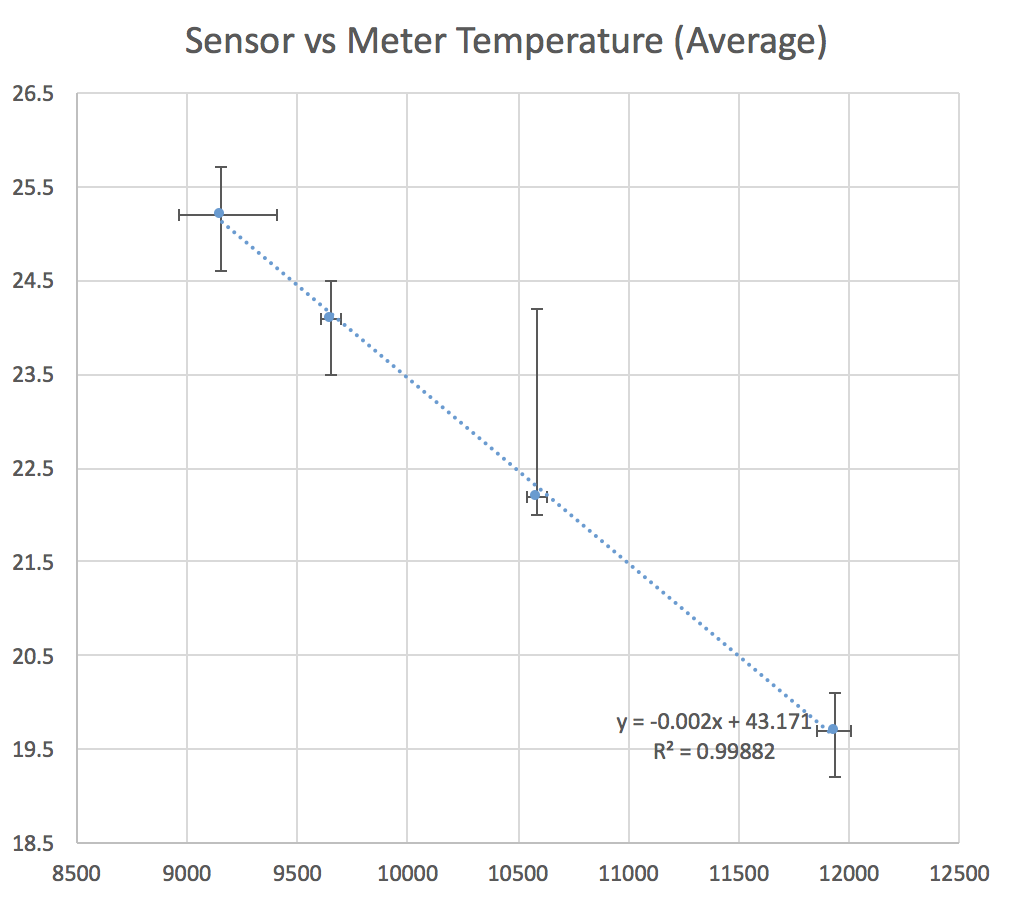
\includegraphics[width=0.75\linewidth]{images/tempcal2.png}
\caption{Detailed calibration of temperature values.}
\label{fig:tempcal2}
\end{figure}

Figure~\ref{fig:tempcal2} shows how the raw sensor values were related to measured temperature values from the meter. Once the bitmask was applied, the linear relationship was evident.

\section{Application Development}

The next step involved developing an Android application using the information found through reverse-engineering the NfcV protocol. The standard Java stack for Android was used, and the resulting application can be seen in Figure~\ref{fig:librejazzpic}.

\begin{figure}[ht]
\centering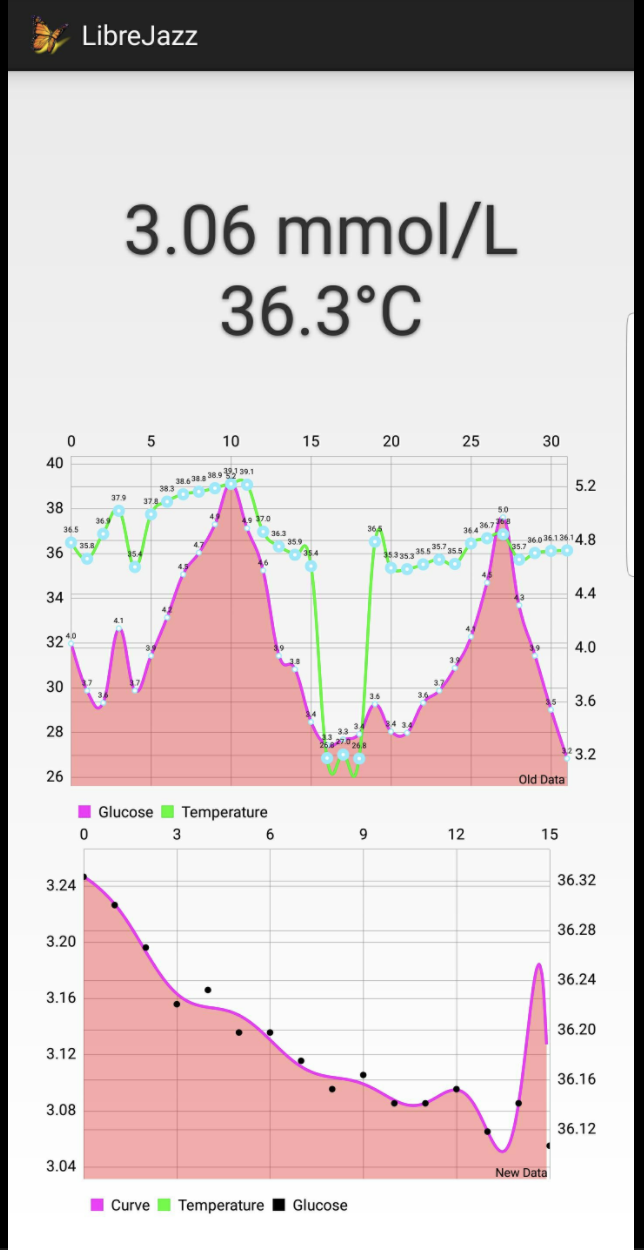
\includegraphics[width=0.35\linewidth]{images/librejazzpic.png}
\caption{Android application for reading sensor raw values.}
\label{fig:librejazzpic}
\end{figure}

Some optimizations were made to increase read times beyond state-of-the-art smartphone apps. From a preliminary study, current solutions were unable to get sensor scan times less than 1.5 seconds. This was found to be due to the large memory of the NC chip in the sensor, and the slow read times of the protocol. Information could only be read in packets of eight bytes - scanning the entire chip took over five seconds, and reading valid program memory took over a second.

Reverse engineering the Glimp app (which provided no source code) allowed for decrypting the sensor tag label from the metadata provided by the sensor. The full algorithm is shown in Figure~\ref{fig:sensortagalgo}. The Libre sensor uses a reduced set of alphanumeric characters and some form of compression to encode the sensor label that is printed on the side of each device.

\begin{figure}[ht]
\centering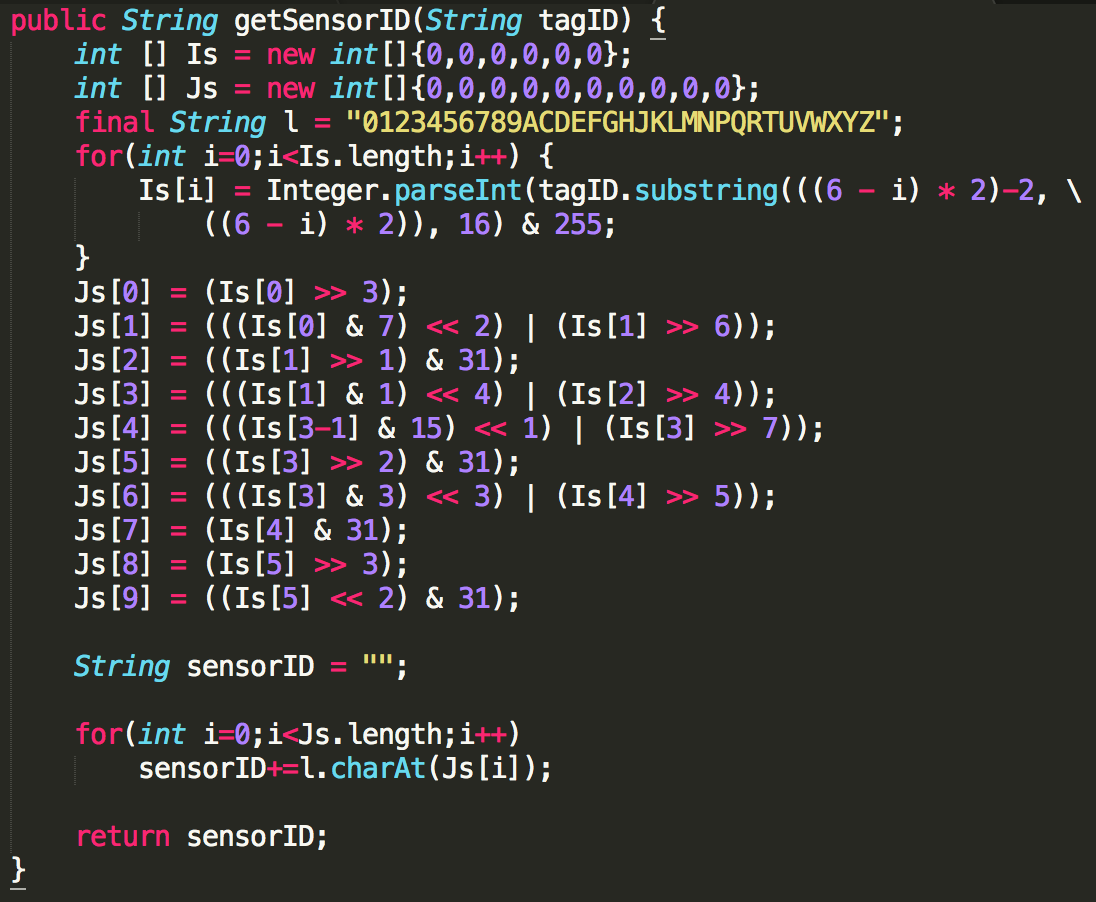
\includegraphics[width=0.75\linewidth]{images/sensortagalgo.png}
\caption{Algorithm used to decrypt sensor tag information.}
\label{fig:sensortagalgo}
\end{figure}

Using this data, it was possible to match previously read values to the values being presently read, and to stop when a previously known value was encountered. This greatly reduced read times by removing the need to read the entire memory, or even the entire array of values. For a subsequent read of the same sensor within 60 seconds, the total read time was less than 50 ms, which only included the time it took to read one short term value and one long term to confirm. On average, read times were decreased to less than 500 ms, which provided a significant advantage over existing apps and systems. The only known faster scanning system is the physical reader provided by Abbott, making this a competitive option due to low cost and greater accessibility.

\section{Reverse Engineering the Reader}
The goal is to get the app to be more accurate to BGM readings, with the Freestyle Libre providing the current gold standard. Our app provides raw sensor data, while BGM readings are straightforward to collect and record. However, we were also hopeful that the Freestyle Libre reader would be able to provide more data.  There had already been significant work towards this. Xavier Claessens reverse engineered many of the previous Abbott devices\cite{claessens_openglucose_2018}. However, most of the prior work reverse engineering the Freestyle Libre was done by Diego Elio Pettenò. He details the reverse engineering journey online\cite{petteno_reverse_2016} and published the finished product GitHub\cite{petteno_glucometer-protocols:_2017}. However, this still does not deliver all the wanted data, so needed further adaption.

The Freestyle Libre is charged by USB and further acts as a USB HID, or Human Interface Device, class. This means it can be queried through libusb for information packets, as when connected to the Abbott software. Mostly through trial and error, the community found two particularly useful commands for data collection. All manual readings - reader spotchecks, blood fingerprick results for glucose and ketones, alongside any associated flags and other information - are returned by the \$arresult command. Interestingly, a historical dataset of values fifteen minutes apart can also be gained, with the \$history command. These correspond to the fifteen minute values stored and returned by the sensor.

Unfortunately, the returned data is heavily obfuscated. It comes in 64-bit packets of hexadecimal dump with a significant amount of noise and no hints of how to identify specific information within the data. Luckily, the necessary parts had already been identified within the community. The code necessary to query the raw data from the reader and map most of the important parts was publicly available\cite{petteno_glucometer-protocols:_2017}. 

In order to end up with the desired data, the device must be queried appropriately, then the returned data must be unobfuscated, separated into instances, and processed. Most of this could be done through the glucometer-utils python code available on GitHub, but needed to be extended to include more information and return in a different format. This was achieved by updating the mapping of the unobfuscated data for each instance, to include date, time, value, sensor runtime, arrow, flags, error and reading type information, where applicable. Processing of time and value was changed, and the formatting was adapted to include the new data in preferred format. This was then easily exported to csv format. 
\chapter{Analysis}

The first objective is to ascertain the algorithm used by the Freestyle Libre reader to arrive at calibrated values, as well as to investigate if this can be improved.

The processed data\footnote{Herein, processed data refers to data collected from the reader, and raw data likewise refers to data directly extracted from the sensor.} - provided by \$history - is distinctly different from the raw  data. As discussed above, the sensor collects data every minute and provides some of this high definition data when scanned. As Figure~\ref{fig:graph3} shows, the processed data is consistently spaced 15 minutes apart, showing that it isn’t merely storage for the raw data. This is emphasized by Figure~\ref{fig:graph3}, which shows that the two datasets clearly don’t match. Most likely, the processed data is a processed version of the 15 minute raw data. Alternatively, the reader may process all raw data, including the high definition, then discard the extras to save space. Both have the same result; all data stored on the reader has been processed.

\begin{figure}[ht]
\centering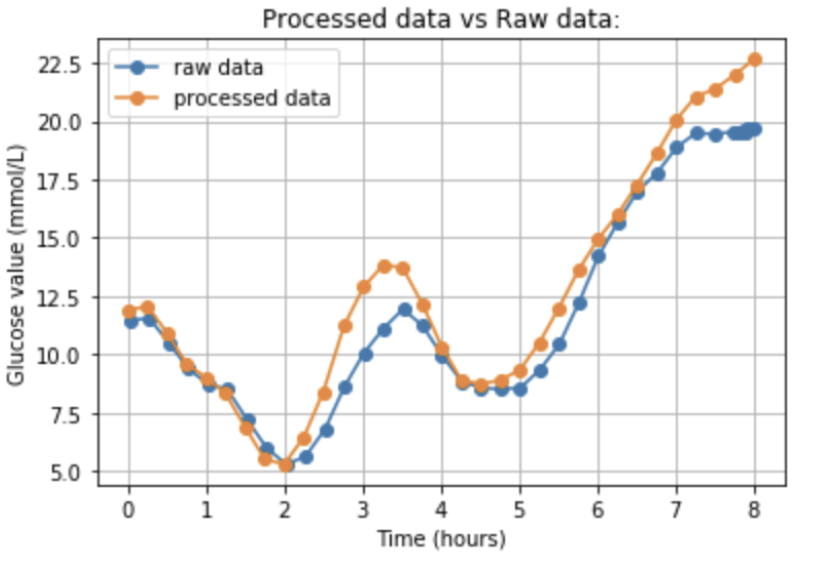
\includegraphics[width=1.0\linewidth]{images/graph3.png}
\caption{Graph of processed(reader) and raw(sensor) data.}
\label{fig:graph3}
\end{figure}

The data displayed on demand with each scan is intended to estimate the current blood glucose level - let's call this read-time data (alternatively manual data, since it is affected by the manual scanning of the sensor). It is clearly formulated from either or both of the processed and raw data. Surprisingly, the processing is not the same as for the other processed data. As seen in Figure~\ref{fig:graph4}, the manually pulled values heavily deviate from the other processed data. The most obvious reason for this would be an attempt to make up for the time lag between interstitial fluid and blood glucose. On the other hand, this could also be part of the initial formula for the processed data, which Figure~\ref{fig:graph3} would appear to support. Another option is that, if the processed data is calculated solely off of 15 minute data, the manual data is different because it also factors in the higher definition one minute data. 

\begin{figure}[ht]
\centering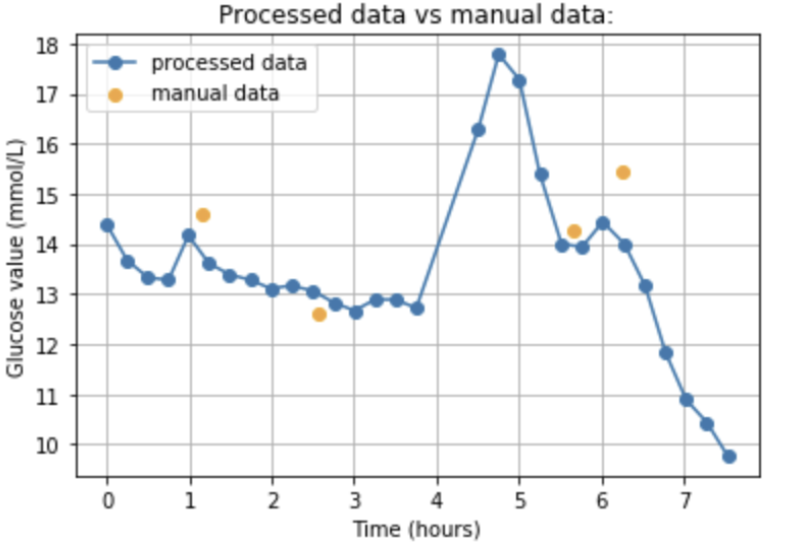
\includegraphics[width=1.0\linewidth]{images/graph4.png}
\caption{Graph of read-time reader data.}
\label{fig:graph4}
\end{figure}

We lacked the data to do a proper accuracy evaluation, and many papers have already done so. However, when graphing the limited blood glucose (fingerprick or \textit{ground truth}) readings against the available time data, as in Figure~\ref{fig:graph0}, some things were notable. The Freestyle Libre was usually reasonably accurate, but was sometimes wildly off. These egregious errors were usually underestimates of a particularly high blood glucose reading. Otherwise it tended to read accurately, even when glucose was changing quickly. The processed reader values were more accurate than the raw values, as expected. Where applicable, the manual readings were usually a bit closer still. Of course, there isn’t enough data to conclusively support any of that.

\begin{figure}[ht]
\centering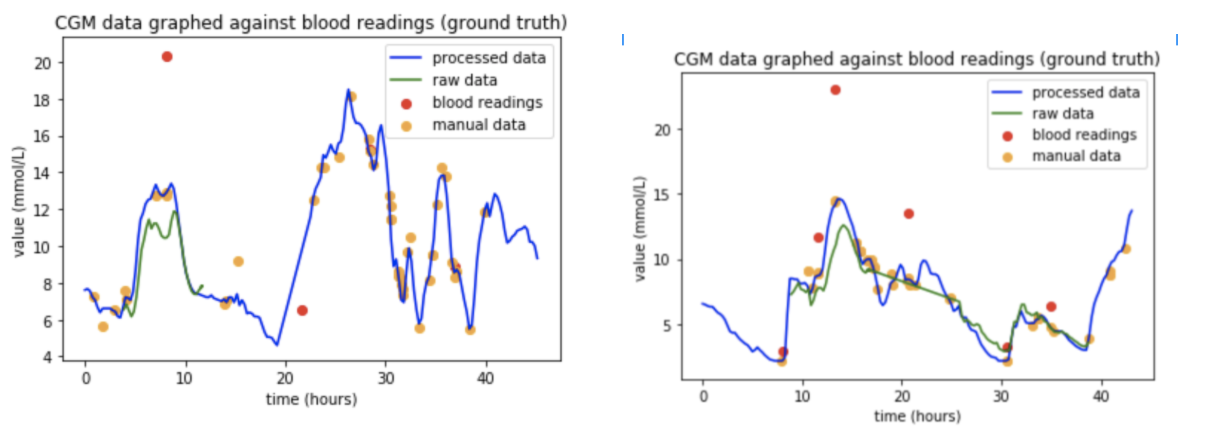
\includegraphics[width=1.0\linewidth]{images/graph0.png}
\caption{Multiple graphs comparing blood glucose data with CGM.}
\label{fig:graph0}
\end{figure}

\section{Prediction}
One of the major additional features that a CGM brings is an element of prediction through data analysis. Improving accuracy of this is very helpful. As previously explained, Freestyle Libre communicates predictions with arrows (see Figure~\ref{fig:arrows}), which translate to the direction glucose is currently trending in mmol/L per minute. First, the accuracy of this needed to be evaluated. The majority of the data we had came in fifteen minute intervals, but it was simple arithmetic to translate the arrow meaning into mmol/L per 15 minute. Matching the time of each manual scan (and hence arrow) to the closest 15 minute change in processed data, an acceptable ground truth, allowed me to get the accuracy of the Freestyle Libre arrows. Depending on the time frame, this varied around 63\% +-5. This seemed fairly low, so effort was made to improve on it using both least squares linear regression and neural networks.

\subsection{Linear Regression}
The initial attempt at linear regression was at seeing whether curve fitting data could be extended to predict future values. As Figure~\ref{fig:graph6} shows, this was predictably unsuccessful. Extending the curve quickly got out of hand, with even the first values being very poorly fit. 

\begin{figure}[ht]
\centering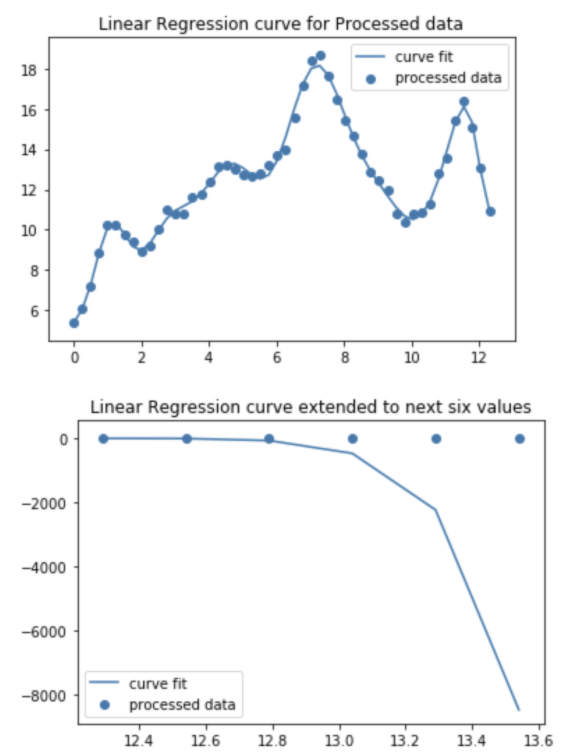
\includegraphics[width=1.0\linewidth]{images/graph6.png}
\caption{Linear Regression results.}
\label{fig:graph6}
\end{figure}

Next, I tried predicting the change in value based on the past 20 datapoints. This initially seemed far more successful than the prior attempt, and even than the reader itself, as shown in Figure~\ref{fig:graph6_5}. The accuracy was taken from testing with separate data, not the training set. While there was some fluctuation depending on the training/test sets chosen, it was consistently above 70\%. Attempting to improve on this - to predict over an hour, to take derivative values as input, to add prior - made little improvement, or caused a backtrack. Nevertheless, it seemed pretty successful.

\begin{figure}[ht]
\centering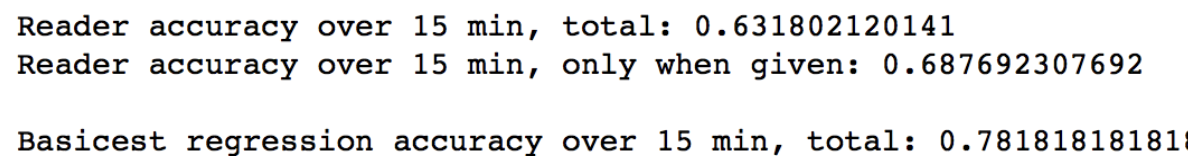
\includegraphics[width=1.0\linewidth]{images/graph6_5.png}
\caption{Linear Regression results on prediction.}
\label{fig:graph6_5}
\end{figure}

\subsection{Neural Networks}
The next attempt at improving on the prediction arrow was a basic neural network, which I expected to be quite successful. However, it would always immediately go to 78\% accuracy and refuse to move through epochs or re-runs, as in Figure~\ref{fig:graph7}. It fluctuated somewhat depending on the testing data, but it was generally settled. This behaviour seemed strange, so I looked further into it.

\begin{figure}[ht]
\centering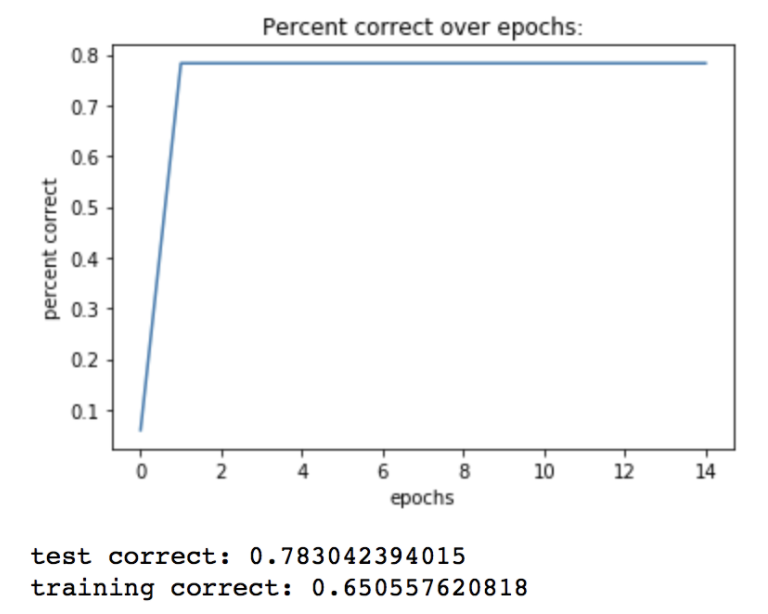
\includegraphics[width=1.0\linewidth]{images/graph7.png}
\caption{Training error against epoch for neural network.}
\label{fig:graph7}
\end{figure}

As it turned out, the problem was that the data was generally too easy to predict. Averaging $\frac{3}{4}$ of it was going straight. This meant the neural network was just persistently returning \textit{straight}, getting it right most of the time, and not changing. In fact, looking back at the linear regression, it suffered the same fault. As Figure~\ref{fig:graph8} shows, the ground truth for the change in value varied between -4 and 4, albeit heavily clustered around zero. The prediction, on the other hand, remains tightly between -1 and 1. This means it still captures most of the data accurately, but ignores two thirds of the possible range.

\begin{figure}[ht]
\centering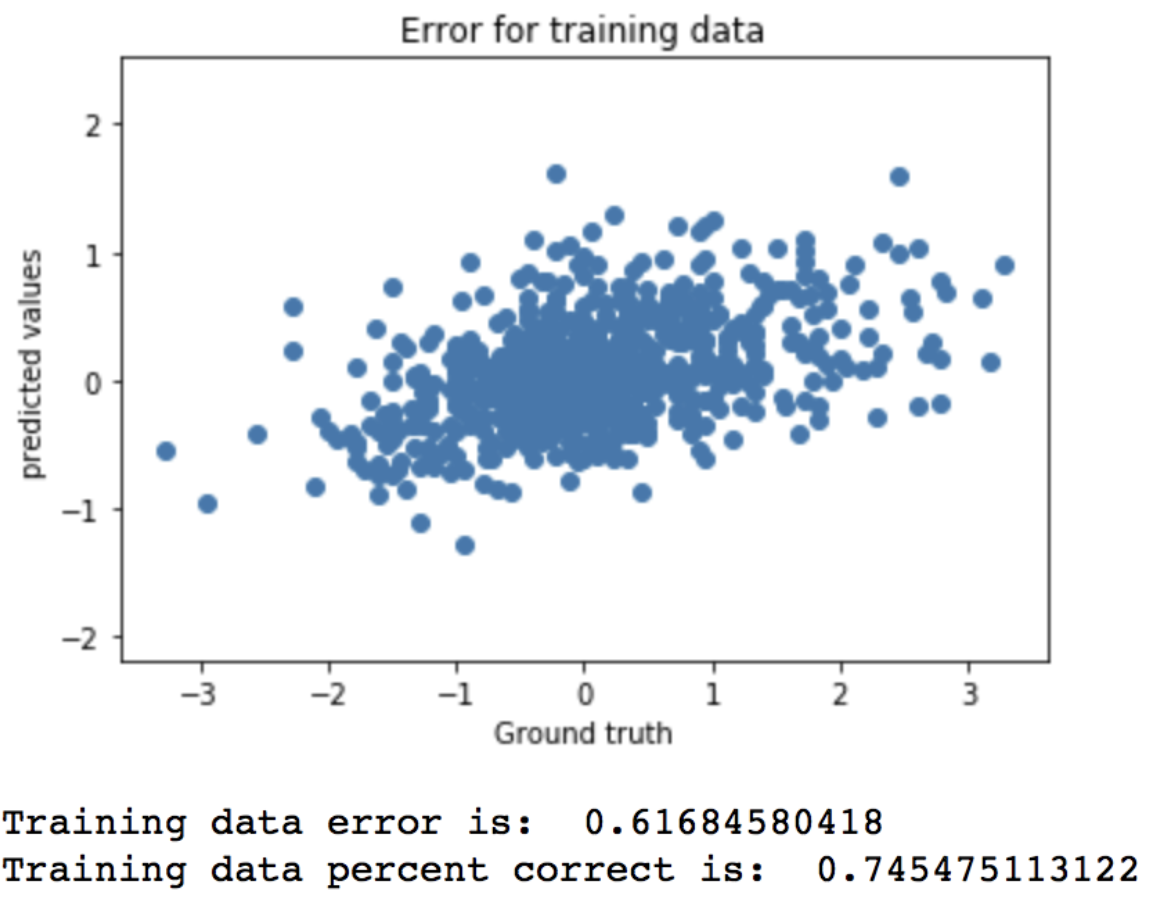
\includegraphics[width=1.0\linewidth]{images/graph8.png}
\caption{Correlation data for prediction.}
\label{fig:graph8}
\end{figure}

\subsection{Reader Prediction Arrow}
The reader’s glucose trend arrow had a poorer mathematical accuracy than either of my algorithms, while displaying the full range of directions instead of just straight. To better understand how this went, I broke down their correct and incorrect instances, as shown in Figure~\ref{fig:graph9}. This shows the distribution of the correct matches, the incorrect arrows, and the incorrectly represented ground truths across the trend directions; the distribution of the differences between a displayed arrow and the corresponding true direction, and a more detailed breakdown of the errors. These numbers tell us a few things.

\begin{figure}[h]
\centering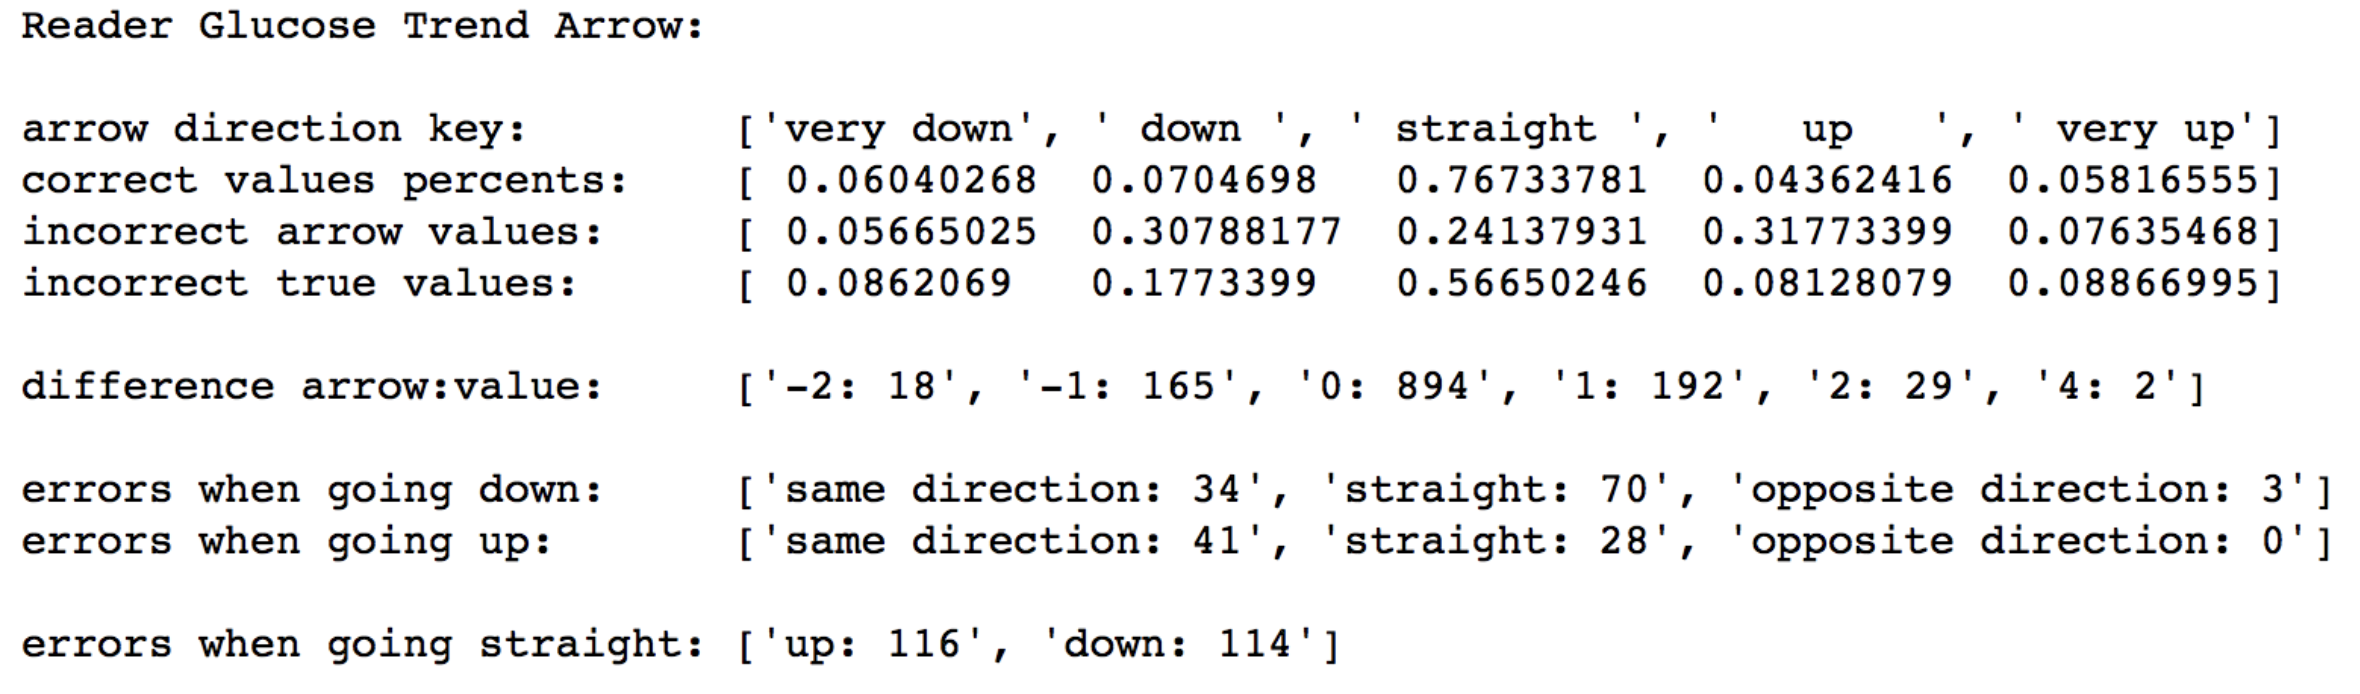
\includegraphics[width=1.0\linewidth]{images/graph9.png}
\caption{Trend arrow statistics.}
\label{fig:graph9}
\end{figure}

First, while the reader is often inaccurate, it’s rarely completely incorrect. Almost 93\% of the predictions is within one degree of the ground truth. Less than 2\% is further away than two degrees. On the other hand, that 2\% is an extreme enough difference to possibly cause harmful management decisions (eg: the difference between 4.2 going straight down, and going straight up). 

The reader exaggerates change. When the reader is correct, it displays a straight arrow 77\% of the time. When the reader is incorrect, it is much more likely to be signalling a change in glucose, only showing straight 24\% of the time. This suggests that the reader algorithm is more responsive to changes in blood glucose than steadiness, and is likely to over exaggerate change in blood glucose. This is in direct contrast to my attempts, which actively conformed everything to ‘straight’, so all the incorrect values were due to rapidly changing bloods being typed as ‘straight’ nonetheless.

On the other hand, the true gradient is more likely to be changing when the reader is incorrect. When the reader was incorrect, the gradient was changing 44\% of the time. This is almost twice the amount when the reader was correct, 23\%. The reader is more likely to read incorrectly on a quickly changing value. Some of this might be overestimating the rate of change, but the rest will be due to underestimating the change. This is in contrast to the early statistics, which suggested that the reader perpetually overestimated change.

With the incorrect readings, the distribution of the true gradient was slightly skewed down. The given arrow value was slightly skewed up. This suggests the reader is more likely to incorrectly predict a higher gradient.

Of the errors that occur while the true value is straight, the uncertainty is very equally distributed between over and underestimating. This suggests a lack of bias. Similarly, the reader has only pointed in completely the wrong direction once. 

When true trend is going down, 60\% of the reader’s incorrect predictions go straight. Only 30\% of the time will an incorrect arrow get the direction, at least, correct. In contrast, if the true trend is up, an incorrect prediction is 60\% likely to be in the right direction, just with the wrong severity. The suggests that the reader arrow exaggerates upwards trends and downplays downwards trends.

The reader’s glucose trend arrow has avoided the trap of only ever predicting straight, while maintaining decent accuracy ratings. It appears to do this by magnifying any change there is in the trend, often resulting in incorrectly predicting more change than there is.



\chapter{Appendix}

All source code and data are located at the primary repo for this paper - \url{https://github.com/hrishioa/Juventas}

\section{Source Code Organization}

Primary organization of the source code is split into three folders: Code, Data and Paper. The \textbf{Code} folder contains all of the applications and utilities written and used for the paper, the \textbf{Data} folder contains raw data read from multiple versions of the Libre app, along with Liapp and Glimp. The \textbf{Paper} folder, understandably contains the tex files used to generate this paper as a form of paperception.

Below are the utilities and scripts included in the \textbf{Code} folder:

\begin{itemize}

\item \textbf{BGMLogger} is a handy script for manually logging blood glucose and tagging information, and produces an output to csv. Usage: \texttt{python BGMLogger.py <filename - default is BGMlog.csv>}

\item \textbf{apk-reverse-engineer} contains all of the files used in the reverse engineering process of the Glimp and Liapp applications. Here the binaries of \textbf{dex2jar} and \textbf{apktool} are included for repeatability, as well as extracted source code and recompiled binaries. Tread at your own risk.

\item \textbf{glucometerutils} is a fork of \cite{petteno_glucometerutils:_2018}, with some modifications added to make logging to csv easier for proper debugging. Some fixes were made to improve performance with the Freestyle Libre, and some locks were removed to improve debugging verbosity\footnote{Please check \url{https://github.com/flameeyes/glucometerutils} for dependencies and usage}. 

\item \textbf{Juventus App} is the Android developed as part of the paper. It is functioning as of the time of writing, and the repository contains the gradle files needed to import and compile in Android Studio, as well as a pre-built apk that will work on Android Versions 17 and up.

\item \textbf{Misc Utilities} contains processing scripts, and may therefore be more cluttered than the rest. The contents are - 

\begin{enumerate}

\item \textbf{glimp\_process.py} can be used to fix unicode errors and patch missing data from the output of \texttt{glucometerutils}. Usage: \texttt{python glimp\_process.py <input\_file> <output\_file>}

\item \texttt{processNFCcsv.py} parses the csv hex dumps from the Android app (disabled by default for performance) to compute glucose and temperature information for testing. The color added console output seen in Figure~\ref{fig:diff} is also produced by this script. The input filename is stored in the script and will need to be modified.

\item \texttt{processrawNFC.py} is very helpful is extracting information directly from the sensor, and therefore is more versatile when used on different sensor. The input is a xml hex dump from NXP TagInfo, which is freely available for Android smartphones. Bypassing any other application dedicated to blood sugar also allows for independent algorithm confirmation. Same as before, the input filename is stored in the script and will need to be modified.

\item \texttt{Graphing.ipynb} is the Jupiter notebook containing raw glucose and temperature plots as well as some sanitization functions for datasets.

\end{enumerate}

\item \textbf{Data} contains all of the raw data used in this experiment. Most common organisation is as a csv, with self-explanatory headings.

\end{itemize}
\newpage

% --------------------------
% Back matter
% --------------------------
{%
\setstretch{1.1}
\renewcommand{\bibfont}{\normalfont\small}
\setlength{\biblabelsep}{0pt}
\setlength{\bibitemsep}{0.5\baselineskip plus 0.5\baselineskip}
\printbibliography
% \printbibliography[nottype=online]
% \printbibliography[heading=subbibliography,title={Websites},type=online,prefixnumbers={@}] 
}
% \cleardoublepage

% \listoffigures
% \cleardoublepage

% \listoftables
% \cleardoublepage

% \newpage
% \mbox{}

% **************************************************
% End of Document CONTENT
% **************************************************
\end{document}
